\documentclass[12pt]{article}

\usepackage[a4paper,  top=1.3in, bottom=1.5in, left=1.5in, right=1.5in]{geometry}

\usepackage[utf8]{inputenc}
\usepackage[T1]{fontenc}
\usepackage{amsmath}
\usepackage{amsfonts}
\usepackage{amssymb}


\usepackage{graphicx, float}
\usepackage{adjustbox}
\graphicspath{{images/}}


%---------------- for graphs ----------------
\usepackage{tikz}
\usepackage{listofitems} % for \readlist to create arrays
\usetikzlibrary{arrows.meta} % for arrow size
\usepackage[outline]{contour} % glow around text
\contourlength{1.4pt}

% COLORS
\usepackage{xcolor}
\colorlet{myred}{red!80!black}
\colorlet{myblue}{blue!80!black}
\colorlet{mygreen}{green!60!black}
\colorlet{myorange}{orange!70!red!60!black}
\colorlet{mydarkred}{red!30!black}
\colorlet{mydarkblue}{blue!40!black}
\colorlet{mydarkgreen}{green!30!black}

% STYLES
\tikzset{
  >=latex, % for default LaTeX arrow head
  node/.style={thick,circle,draw=myblue,minimum size=22,inner sep=0.5,outer sep=0.6},
  node in/.style={node,green!20!black,draw=mygreen!30!black,fill=mygreen!25},
  node hidden/.style={node,blue!20!black,draw=myblue!30!black,fill=myblue!20},
  node convol/.style={node,orange!20!black,draw=myorange!30!black,fill=myorange!20},
  node out/.style={node,red!20!black,draw=myred!30!black,fill=myred!20},
  connect/.style={thick,mydarkblue}, %,line cap=round
  connect arrow/.style={-{Latex[length=4,width=3.5]},thick,mydarkblue,shorten <=0.5,shorten >=1},
  node 1/.style={node in}, % node styles, numbered for easy mapping with \nstyle
  node 2/.style={node hidden},
  node 3/.style={node out}
}
\def\nstyle{int(\lay<\Nnodlen?min(2,\lay):3)} % map layer number onto 1, 2, or 3


\tikzset{basic/.style={draw,fill=none,
                       text badly centered,minimum width=3em}}
\tikzset{input/.style={basic,circle,minimum width=3.5em}}
\tikzset{weights/.style={basic,rectangle,minimum width=2em}}
\tikzset{functions/.style={basic,circle, minimum width=4em}}
\newcommand{\addaxes}{\draw (0em,1em) -- (0em,-1em)
                            (-1em,0em) -- (1em,0em);}
\newcommand{\relu}{\draw[line width=1.5pt] (-1em,0) -- (0,0)
                                (0,0) -- (0.75em,0.75em);}
\newcommand{\stepfunc}{\draw[line width=1.5pt] (0.65em,0.65em) -- (0,0.65em) 
                                    -- (0,-0.65em) -- (-0.65em,-0.65em);}

%-----------------------------------------------------


\renewcommand{\figurename}{Slika}



\renewcommand{\baselinestretch}{1.2} % Line spacing

% Parskip and parindent
\setlength{\parindent}{0pt} % Begin of paragraph indentation
\setlength{\parskip}{1em} % Paragraph spacing

%--- for references ---------
\usepackage[
   backend=biber,
   style=numeric,
   sorting=none
   ]{biblatex}

\addbibresource{bibliography.bib}
\AtBeginBibliography{\vspace*{10pt}}
%----------------------------

%----------- toc ------------------------
\usepackage{tocloft}
\usepackage{fancyhdr}
% \setlength{\cftbeforesecskip}{0pt} % Adjust the spacing before section entries
% \setlength{\cftbeforesubsecskip}{0pt} % Adjust the spacing before subsection entries
%----------------------------------------

\begin{document}

   % Title Page
   \newgeometry{top=1in, bottom=1in, left=1in, right=1in} % New margins for title page
   \begin{titlepage}
      \begin{center}
         
         % add your university logo here
         % negative value moves the logo up
         \vspace*{-1in}
         
\includegraphics[width=0.4\textwidth]{raf_logo.png}

         % set font size to 14pt
         \vspace{1in}
         \Large
         \textbf{DIPLOMSKI RAD}
         
         % set horizontal margin for the title to 1.5in and center it
         \vspace{1in}
         \Huge
         \textbf{Slika je vredna 16x16 reči: \\ Vision Transformeri}
         
         \vspace{1in}


         \fontsize{14pt}{18pt}\selectfont
         \textbf{Vanja Kovinić} \\
         \textbf{RN 42/2020}
         \vspace*{1.5in}
         
         \begin{center}
            \normalsize
            \begin{tabular}{p{0.7\textwidth} p{0.5\textwidth}}
               \fontsize{14pt}{18pt}\selectfont   
               \textbf{Mentor:} & 
            
               \fontsize{14pt}{18pt}\selectfont
               \textbf{Komisija:} \\
               dr Nemanja Ilić & dr Nemanja Ilić \\
                                 & dr Nevena Marić \\
            \end{tabular}
         \end{center}

         \vspace*{\fill}

         \normalsize
         Beograd, septembar 2024.


         
      \end{center}
   \end{titlepage}
   \restoregeometry % Restore original margins

   \newpage
   \newgeometry{top=1.3in, bottom=2.2in, left=1.4in, right=1.4in} % New margins for title page
   
   % Table of Contents
   \renewcommand{\contentsname}{Sadržaj}
   \addtocontents{toc}{\protect\thispagestyle{empty}}
   \tableofcontents
   \thispagestyle{empty} % Remove page numbers

   \restoregeometry % Restore original margins
   \newpage
   
   \thispagestyle{empty} % Remove page number from Abstract page

   % Define a command to format a specific section title
   \newcommand{\specialsection}[1]{
      \section*{\centering{#1}} % Center and italicize the section title
   }

   \vspace*{0.5in}
   \specialsection{Apstrakt}
   

   \vspace*{0.5in}

   Ovaj diplomski rad istražuje \textbf{Vision Transformere} (\textbf{ViT}),
   nov pristup u oblasti računarskog vida koji koristi arhitekturu
   transformera prvobitno razvijenu za obradu prirodnog jezika. Prvi deo rada pruža detaljan pregled arhitekture transformera, 
   uključujući ključne komponente kao što su \textbf{\textit{self-attention} mehanizam} i \textbf{poziciono enkodovanje},
   i diskutuje njihove svrhe i funkcionalnosti. Nakon toga, fokus se prebacuje
   na Vision Transformere, objašnjavajući kako se slike transformišu
   u \textbf{tokene} i obrađuju kroz \textbf{enkoder transformera} kako bi se primenili na rešavanje vizuelnih zadataka.

   Rad zatim ulazi u praktične aspekte implementacije Vision Transformera,
   uključujući izbor i podešavanje \textbf{hiperparametara} za poboljšanje performansi.
   Izvršeno je i poređenje sa referentnim implementacijama, i predložen pristup za 
   poboljšanje performansi. Prikazani su različiti
   eksperimenti, zajedno sa diskusijom njihovih rezultata, pružajući uvid
   u efikasnost i izazove povezane sa Vision Transformerima.

   % Na kraju, rad naglašava značaj Vision Transformera u oblasti računarskog vida, 
   % prikazujući njihov potencijal i ograničenja, kao i njihove praktične primene.

   \newpage
   \pagenumbering{arabic}
   \setcounter{page}{1}

   \section{Uvod}
   
   \textit{"Pre otprilike 540 miliona godina, 
   Zemlja je bila obavijena tamom.
   Ovo nije bilo zbog nedostatka svetlosti,
   već zato što organizmi još uvek nisu razvili sposobnost da vide.
   Iako je sunčeva svetlost mogla da prodre u okeane do dubine
   od 1.000 metara i hidrotermalni izvori na dnu mora isijavali 
   svetlost u kojoj je život cvetao, nijedno oko nije se moglo naći 
   u tim drevnim okeanima, nijedna retina, rožnjača ili sočivo. 
   Sva svetlost i život nikada nisu viđeni. Koncept gledanja nije ni postojao tada 
   i ova sposobnost nije ostvarena sve dok nije stvorena.
   }
   
   \textit{Iz nama nepoznatih razloga, trilobiti su se pojavili kao prva bića sposobna
   da spoznaju svetlost. Oni su prvi prepoznali da postoji nešto izvan
   njih samih, svet okružen višestrukim jedinkama. Smatra se da je rađanje vida pokrenulo
   kambrijsku eksploziju, period u kojem se veliki broj vrsta životinja pojavljuje u 
   fosilnom zapisu. Vid je započeo kao pasivno iskustvo, jednostavno propuštanje svetlosti, 
   ali je ubrzo postao aktivniji. Nervni sistem je počeo da evoluira, vid je prešao u uvid, 
   gledanje je postalo razumevanje, razumevanje je dovelo do akcije, a sve to je dovelo do 
   nastanka inteligencije.}
   
   \textit{Danas nismo više zadovoljni vizuelnom spoznajom koju nam je priroda dala. 
   Radoznalost nas je navela da stvorimo mašine koje mogu da "vide" kao mi, pa čak i inteligentnije."} - Li Fei-Fei \cite{li_fei_fei}
   

   \subsection{Istorija i motivacija}
   \vspace{-0.5cm}
   \subsubsection{Rani Razvoj u Računarskom Vidu}

   Koreni računarskog vida potiču iz ranih pokušaja da se razume 
   i interpretira vizuelni podatak korišćenjem matematičkih modela i računara. 
   U početku, istraživanja u oblasti računarskog vida fokusirala su se na 
   jednostavne zadatke kao što su detekcija ivica, prepoznavanje objekata i 
   osnovna obrada slika. Rane metode su se u velikoj meri oslanjale na ručnu 
   izradu karakteristika (eng. \textbf{\textit{features}}) slike i algoritme dizajnirane da imitiraju osnovne aspekte 
   ljudskog vida.

   \subsubsection{Uspon Dubokog Učenja}

   Značajan preokret u računarskom vidu dogodio se sa pojavom \textbf{dubokog učenja}. 
   \textbf{Konvolucione Neuronske Mreže} (eng. \textbf{CNN}), koje su predstavili Yann LeCun i drugi \cite{lecun_cnn} 
   krajem 1980-ih i početkom 1990-ih, transformisale su ovu oblast uvođenjem automatskog 
   ekstraktovanja karakteristika kroz slojeve koji se uče (eng. \textbf{\textit{learnable features}}). \textbf{CNN}-ovi su pokazali izuzetne 
   performanse u različitim zadacima klasifikacije slika, omogućavajući računarima da 
   nauče složene reprezentacije vizuelnih podataka. Ovo otkriće je kasnije propraćeno uspehom modela 
   kao što su \textbf{AlexNet} \cite{alexnet}, \textbf{VGGNet} \cite{vgg} i \textbf{ResNet} \cite{resnet}, koji su postavili nove standarde u izazovima 
   prepoznavanja slika.

   \subsubsection{Ograničenja CNN-ova}

   Uprkos svom uspehu, \textbf{CNN}-ovi imaju inherentna ograničenja \cite{cnn_limits} 
   koja su motivisala potragu za novim pristupima. Jedan od 
   značajnih nedostataka je njihova poteškoća u modelovanju udaljenih zavisnosti
   i globalnog konteksta unutar slike. \textbf{CNN}-ovi obično obrađuju slike kroz seriju 
   lokalizovanih konvolucionih operacija, što može ograničiti njihovu sposobnost da 
   razumeju odnose između udaljenih elemenata na slici.

   \subsubsection{Motivacija za uvođenje Vision Transformera}

   Pojava \textbf{Vision Transformera} (\textbf{ViT}) predstavlja odgovor na ova ograničenja. 
   Inspirisani uspehom modela transformera u obradi prirodnog jezika (\textbf{NLP}), 
   istraživači su pokušali da primene iste principe u računarskom vidu \cite{vit}. 
   Transformeri koriste \textbf{\textit{self-attention}} mehanizam za povezivanje globalnih zavisnosti, 
   što ih čini pogodnim za zadatke koji zahtevaju razumevanje 
   složenih odnosa unutar vizuelnih podataka.
   
   \newpage

   \textbf{Vision Transformeri} rešavaju nekoliko izazova sa kojima se suočavaju \textbf{CNN}-ovi. 
   Pretvaranjem slika u sekvence parčića (eng. \textbf{\textit{image patches}}) i primenom \textit{self-attention} mehanizma preuzetim iz transformera, 
   \textbf{ViT}-ovima mogu efikasnije modelovati globalni kontekst. 
   Ovaj pristup omogućava \textbf{ViT}-ovima da postignu vrhunske performanse na različitim  
   testovima klasifikacije slika i pokazuje njihov potencijal da unaprede oblast računarskog vida \cite{vit}.

   \subsection{Konvolucione Neuronske Mreže (CNN)}
   \subsubsection{Istorija CNN-ova}
   Konvolucione neuronske mreže su razvijene 
   i prvi put korišćene oko 1980-ih. Tokom tog perioda, primarna primena 
   \textbf{CNN}-ova bila je prepoznavanje rukom pisanih cifara, što je našlo 
   praktičnu primenu u poštanskom sektoru za čitanje poštanskih i PIN kodova. 
   Rani modeli \textbf{CNN}-ova, kao što je \textbf{LeNet} \cite{lenet} koji je razvio Yann LeCun, pokazali su 
   potencijal CNN-ova za zadatke prepoznavanja cifara \cite{cnn_history}.

   Međutim, šira primena \textbf{CNN}-ova bila je ograničena značajnim izazovima. 
   Duboki modeli učenja, uključujući \textbf{CNN}-ove, zahtevaju ogromne količine 
   podataka za obuku i značajne računarske resurse, koji u to vreme nisu 
   bili lako dostupni. Pored toga, \textbf{\textit{backpropagation}} algoritam, 
   koji je neophodan za obuku neuronskih mreža, bio je računarski skup. 
   Ova ograničenja su suzila upotrebu \textbf{CNN}-ova uglavnom na poštanski sektor, 
   i tehnologija nije uspela da stekne širu primenu u oblasti mašinskog učenja \cite{cnn_history_2}.

   Oživljavanje \textbf{CNN}-ova došlo je 2012. godine, kada su Alex Krizhevsky, zajedno 
   sa Ilyom Sutskeverom i Geoffreyjem Hintonom, prepoznali potencijal dubokog 
   učenja sa višeslojnim neuronskim mrežama. Ovo oživljavanje je pokrenuto od strane nekoliko 
   ključnih faktora: dostupnost velikih skupova podataka, kao što je \textbf{\textit{ImageNet}} \cite{imagenet} skup sa 
   milionima označenih slika, i značajna unapređenja u računarskim resursima, posebno \textbf{GPU}-ovima 
   (eng. \textbf{\textit{graphics processing unit}}). Ovi razvojni događaji omogućili su istraživačima da prevaziđu prethodna ograničenja i u 
   potpunosti iskoriste mogućnosti konvolucionih neuronskih mreža \cite{cnn_history_2}.

   \subsubsection{Ljudski vizuelni sistem kao inspiracija}
   Arhitektura konvolucionih neuronskih mreža je analogna načinu na koji su neuroni u
   ljudskom mozgu povezani i inspirisana je organizacijom \textbf{vizuelnog korteksa} (\textit{Slika 1}). 
   Pojedinačni neuroni reaguju na stimuluse samo u ograničenom delu vizuelnog polja 
   poznatom kao \textbf{receptivno polje} (eng. \textbf{\textit{receptive field}}). 
   Ova polja se preklapaju kako bi se pokrilo čitavo vizuelno polje.


   \begin{figure}[h!]
      \centering
      \vspace{1.5cm} % Add vertical space
      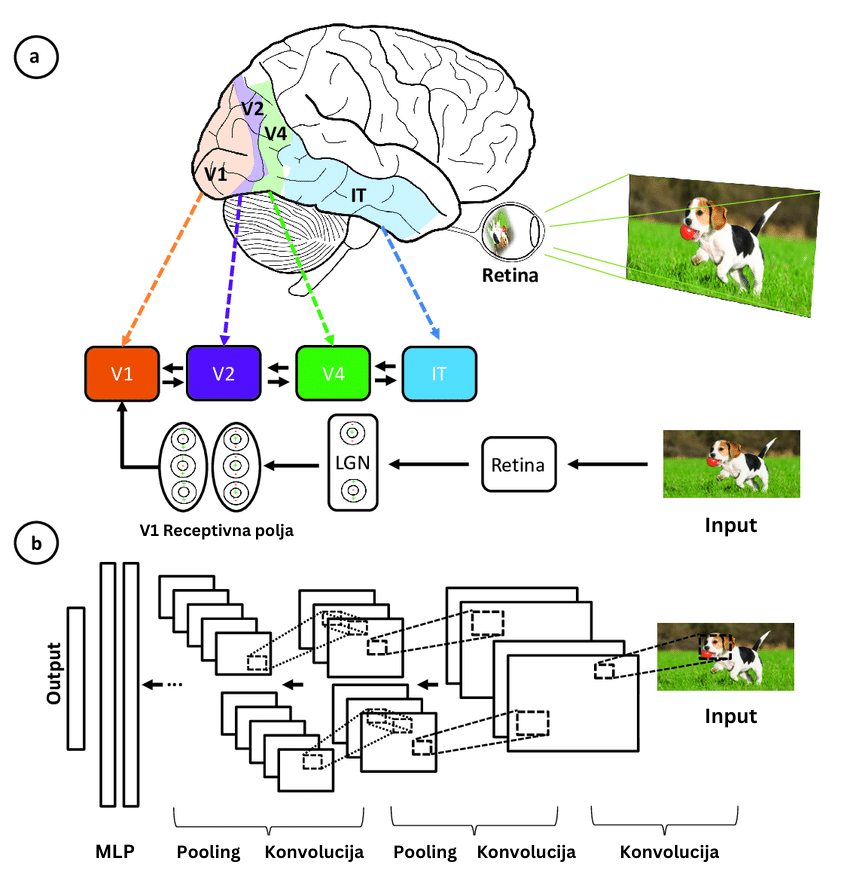
\includegraphics[width=0.8\textwidth]{visual_cortex.png}
      \caption{Poređenje između organizacije vizuelnog korteksa i \textbf{CNN} arhitekture \cite{hvc_pic}}
      \label{fig:visual_cortex}
   \end{figure}

   \newpage

   Prema Keitu \cite{human_visual_cortex}, glavne sličnosti između organizacije vizuelnog korteksa i arhitekture \textbf{CNN}-ova su:
   \begin{itemize}
   \item \textbf{Hijerarhijska arhitektura}: I \textbf{CNN} i vizuelni korteks imaju hijerarhijsku strukturu, 
   gde se jednostavni oblici izvlače u početnim slojevima, a složeniji oblici se grade u dubljim slojevima. 
   Ovo omogućava kompleksniju reprezentaciju vizuelnog inputa.
   \item \textbf{Lokalna povezanost}: Neuroni u vizuelnom korteksu su povezani samo sa 
   lokalnim regionom inputa, a ne sa celim vizuelnim poljem. Slično tome, neuroni 
   u sloju \textbf{CNN}-a su povezani samo sa lokalnim regionom inputa putem \textbf{konvolucione operacije}. 
   Ova lokalna povezanost omogućava efikasnost.
   \item \textbf{Translaciona invarijantnost}: Neuroni vizuelnog korteksa mogu detektovati karakteristike
    bez obzira na njihovu lokaciju u vizuelnom polju. \textbf{\textit{Pooling}} slojevi u \textbf{CNN}-u pružaju određeni 
    stepen \textbf{translacione invarijantnosti}.
    \item \textbf{Višestruke \textit{feature} mape}: Na svakoj fazi vizuelne obrade, izvlače se različite \textbf{\textit{feature}} mape.
    \textbf{CNN}-ovi ovo imitiraju putem višestrukih jezgara (eng. \textbf{\textit{kernels}}) koji detektuju različite karakteristike
      u svakom konvolucionom sloju.
   \item \textbf{Nelinearnost}: Neuroni u vizuelnom korteksu pokazuju osobine nelinearnosti. 
   \textbf{CNN}-ovi postižu nelinearnost putem \textbf{aktivacionih funkcija}, koje se primenjuju nakon svake konvolucije.
   
   \end{itemize}
   
   \newpage

   \subsubsection{Arhitektura CNN-ova}
   Arhitektura \textbf{CNN}-a biće prikazana na primeru klasifikacionog
    problema\footnote{Gradivni elementi CNN-a su identični, bez obzira na to
     da li je u pitanju problem regresione ili neke druge prirode; jedina razlika leži u MLP glavi.}, 
     gde je cilj modela da klasifikuje slike u jednu od $P$ klasa, kao što je prikazano na \textit{Slici 2}.


     \begin{figure}[h!]
      \centering
      \adjustbox{scale=0.45,center}{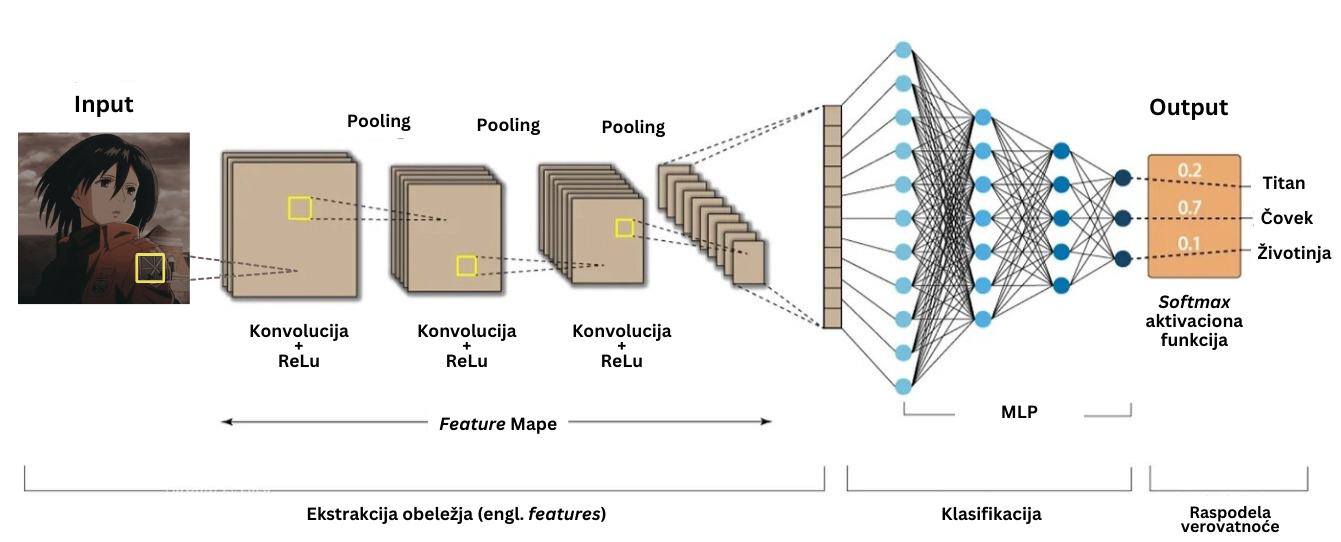
\includegraphics{cnn_arhitecture.png}} % Adjust the scale factor as needed
      \caption{Primer arhitekture \textbf{CNN}-a za klasifikaciju slika}
      \label{fig:cnn_architecture}
    \end{figure}
    
    \vspace{0.7cm}
   
    Sastavni deo \textbf{CNN}-a su:
    \begin{itemize}
      % remove white space between first item and start of the list
      \vspace{-0.5cm}
      \setlength\itemsep{0em}
      \item \textbf{Konvolucioni slojevi}
      \item \textbf{\textit{Pooling} slojevi}
      \item \textbf{Višeslojni perceptron (eng. \textbf{\textit{Multi-Layer Perceptron}} - \textbf{MLP})}
   \end{itemize}

   \newpage

   \subsection*{Konvolucioni slojevi}
   \subsubsection*{1. Konvoluciona operacija}
   U \textbf{konvolucionom sloju}, osnovna operacija je \textbf{konvolucija} ulazne slike sa \textbf{kernelom} (poznatim i kao \textbf{filter}).
   Cilj ove operacije je detektovanje karakteristika kao što su ivice, teksture 
   ili šare u ulaznim podacima.

   Neka je ulazna slika predstavljena kao 2D matrica \( I \) 
   sa dimenzijama \( H \times W \), gde je \( H \) visina, 
   a \( W \) širina slike. Neka je \( K \) 2D kernel sa 
   dimenzijama \( f \times f \), gde je \( f \) veličina kernela.
   
   Operacija konvolucije se može matematički izraziti kao:
   \[
   S(i, j) = \sum_{m=0}^{f-1} \sum_{n=0}^{f-1} I(i+m, j+n) \cdot K(m, n)
   \]
   gde \( S(i, j) \) predstavlja vrednost izlazne \textbf{\textit{feature}} mape na poziciji 
   \((i, j)\). Ovde \( (i, j) \) označava poziciju na ulaznoj slici gde se primenjuje kernel \cite{conv}.

   \subsubsection*{2. Izlaz konvolucione operacije}
   Rezultat primene kernela na ulaznu sliku je \textit{feature} mapa \( F \) 
   sa dimenzijama \((H - f + 1) \times (W - f + 1)\), pod pretpostavkom da se ne 
   koristi \textit{padding} (\textit{Slika 3}). Veličina izlazne \textit{feature} mape je 
   smanjena u odnosu na ulaznu sliku zbog klizne operacije kernela preko ulazne slike.

   \newpage   

   \begin{figure}[h!]
      \centering
      \adjustbox{scale=0.2,center}{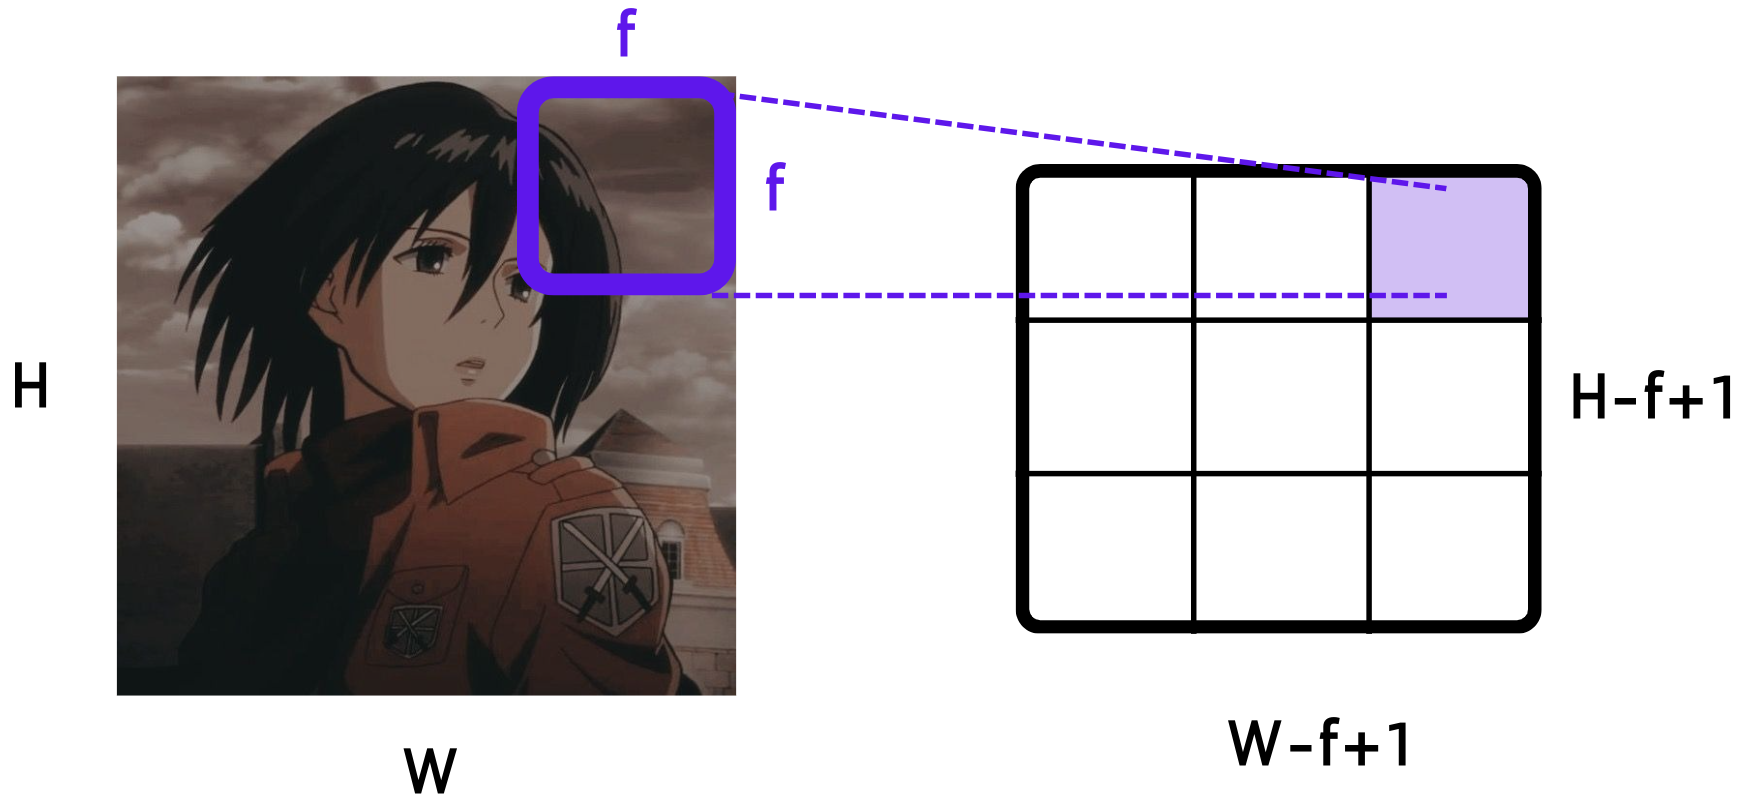
\includegraphics{convolution.png}} % Adjust the scale factor as needed
      \caption{Dimenzije ulazne slike i \textit{feature} mape u jednom konvolucionom sloju}
      \label{fig:convolution}
    \end{figure}

    \subsubsection*{3. Popunjavanje (eng. Padding)}

    Popunjavanje se koristi za kontrolu prostornih dimenzija izlazne \textit{feature} mape \cite{padding}. 
    Popunjavanje predstavlja dodavanje piksele oko ivica ulazne slike. 
    Neka je \( p \) broj piksela koji se dodaju. 
    Popunjena ulazna slika \( I' \) ima dimenzije \((H + 2p) \times (W + 2p)\).
    
    Operacija konvolucije sa popunjavanjem može se izraziti kao:
    \[
    S(i, j) = \sum_{m=0}^{f-1} \sum_{n=0}^{f-1} I'(i+m, j+n) \cdot K(m, n).
    \]

   \subsubsection*{4. Korak (eng. Stride)}
   Korak određuje koliko piksela se filter pomera pri svakom koraku tokom konvolucije \cite{stride}. 
   Neka je \( s \) vrednost koraka. Korak utiče na dimenzije izlazne \textit{feature} mape. 
   Sa korakom \( s \), izlazna \textit{feature} mapa \( F \) ima dimenzije:
   \[
      H_{\text{out}} = \frac{H - f + 2p}{s} + 1
   \]
   \[
   W_{\text{out}} = \frac{W - f + 2p}{s} + 1
   \]
   gde su \( H_{\text{out}} \) i \( W_{\text{out}} \) visina i širina izlazne \textit{feature} mape, 
   respektivno.

   \subsection*{5. Aktivaciona Funkcija}

   Nakon konvolucione operacije, aktivaciona funkcija se primenjuje element po element da bi se 
   uvela nelinearnost u model. Aktivaciona funkcija koja se najčešće koristi je 
   \textbf{ReLU} (\textit{Rectified Linear Unit}), definisana kao:
   \[
   \text{ReLU}(x) = \max(0, x)
   \]
   gde je \( x \) ulaz u aktivacionu funkciju. Neke od najpopularnijih aktivacionih funkcija se mogu 
   videti na \textit{Slici 4}.

   \begin{figure}[h!]
      \centering
      \adjustbox{scale=0.7,center}{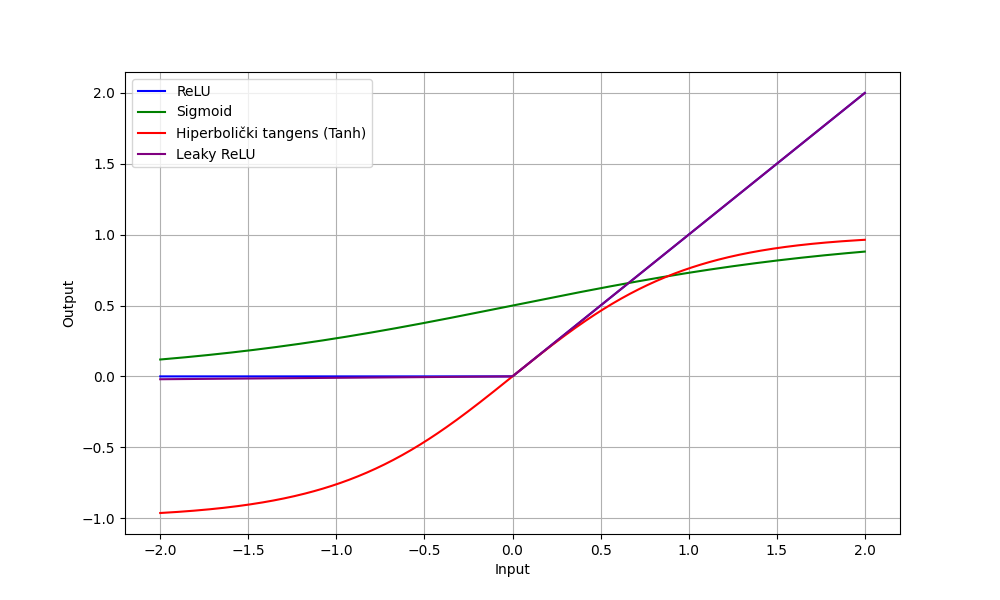
\includegraphics{pop_activations.png}} % Adjust the scale factor as needed
      \caption{Grafik najčešće korišćenih aktivacionih funkcija}
      \label{fig:pop_activations}
    \end{figure}

    \newpage 
    
    \subsection*{Pooling slojevi}
   Pooling slojevi su još jedna ključna komponenta \textbf{CNN}-ova koja vrši operaciju uzorkovanja po određenoj strategiji kako bi 
   se smanjile prostorne dimenzije ulazne \textit{feature} mape, čime se smanjuje 
   računarska složenost i sprečava prekomerno prilagođavanje (eng. \textit{overfitting}). 
   Najčešće korišćene operacije pooling-a su \textbf{\textit{max pooling}} i \textbf{\textit{average pooling}} \cite{pooling}.
   \subsubsection*{Pooling operacija}
   \textit{Pooling} operacije se primenjuju na svaku \textit{feature} mapu nezavisno. 
   Ulazna \textit{feature} mapa \( F \) ima dimenzije \( H \times W \), gde je \( H \) visina, 
   a \( W \) širina. \textit{Pooling} operacija pomera prozor veličine \( f \times f \) preko \textit{feature} mape,
   sa korakom \( s \).
   \subsubsection*{Max Pooling}
   \vspace{-0.3cm}
   Kod \textit{max pooling} operacije, izlazna vrednost za svaki prozor je maksimalna vrednost 
   unutar tog prozora. Matematički, za \textit{feature} mapu \( F \) i \textit{pooling} prozor 
   veličine \( f \times f \) sa korakom \( s \), 
   \textit{max pooling} operacija se može izraziti kao:
   \[
   M(i, j) = \max_{0 \leq m < f, 0 \leq n < f} F(s \cdot i + m, s \cdot j + n)
   \]
   gde \( M(i, j) \) predstavlja vrednost izlazne \textit{feature} mape na poziciji \((i, j)\).
   \subsubsection*{Average Pooling}
   \vspace{-0.3cm}
   Kod \textit{average pooling} operacije, izlazna vrednost za svaki prozor je prosečna vrednost unutar tog 
   prozora. Matematički, za \textit{feature} mapu \( F \) i \textit{pooling} prozor veličine 
   \( f \times f \) sa korakom \( s \), 
   \textit{average pooling} operacija se može izraziti kao:
   \[
   A(i, j) = \frac{1}{f^2} \sum_{m=0}^{f-1} \sum_{n=0}^{f-1} F(s \cdot i + m, s \cdot j + n)
   \]
   gde \( A(i, j) \) predstavlja vrednost izlazne mape karakteristika na poziciji \((i, j)\).

   \newpage
   \subsubsection*{Izlaz Pooling-a}

   Dimenzije izlazne \textit{feature} mape zavise od veličine prozora za pooling \( f \) i koraka \( s \). 
   Za datu ulaznu \textit{feature} mapu \( F \) dimenzija \( H \times W \), izlazna \textit{feature} mapa \( O \) 
   (bilo \( M \) za \textit{max pooling} ili \( A \) za \textit{average pooling}) ima dimenzije:
   
   \[
   H_{\text{out}} = \frac{H - f}{s} + 1
   \]
   \[
   W_{\text{out}} = \frac{W - f}{s} + 1
   \]
   
   gde su \( H_{\text{out}} \) i \( W_{\text{out}} \) visina i širina izlazne \textit{feature} mape, respektivno \\ (ilustracija \textit{pooling} operacije na \textit{Slici 5}).
   
   
   \begin{figure}[h!]
      \centering
      \vspace{0.5cm} % Add vertical space
      \adjustbox{scale=0.7,center}{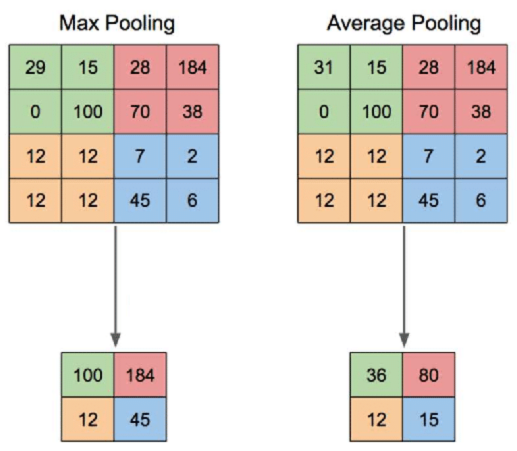
\includegraphics{pooling.png}} % Adjust the scale factor as needed
      \caption{Primer izvođenja \textit{max pooling} i \textit{average pooling} operacije \cite{pooling}}
      \label{fig:max_avg_pooling}
    \end{figure}

    \newpage
   \subsection*{Višeslojni Perceptron (MLP)}
   \subsubsection*{Perceptron}
    \vspace{-0.5cm}
   Perceptron prima više ulaznih signala, primenjuje težine na njih, 
   sabira ih i prosleđuje rezultat kroz aktivacionu funkciju kako bi proizveo izlaz (\textit{Slika 6}).
   
   Za dat ulazni vektor \(\mathbf{x} = [x_0, x_2, \ldots, x_n]\) i odgovarajuće težine 
   $\mathbf{w} = [w_0, w_2,$ $\ldots, w_n]$, perceptron računa ponderisanu sumu na sledeći način:
   \[
   z = \sum_{i=0}^{n} w_i x_i
   \]
   gde je \(x_0=1\), pa je $x_0w_0$ slobodan član (često se još naziva i pomeraj, a obeležava kao $b$, eng. \textit{bias}).
   
   Izlaz \(y\) se zatim dobija primenom aktivacione funkcije \(f(z)\). U našem primeru smo za
   aktivacionu funkciju koristili \textbf{ReLU} funkciju, koja se definiše na sledeći način:
   \[
      y = 
      \begin{cases}
         z, & \text{ako } z > 0 \\
         0, & \text{inače}.
      \end{cases}
      \]
      
      \begin{figure}[h!]
         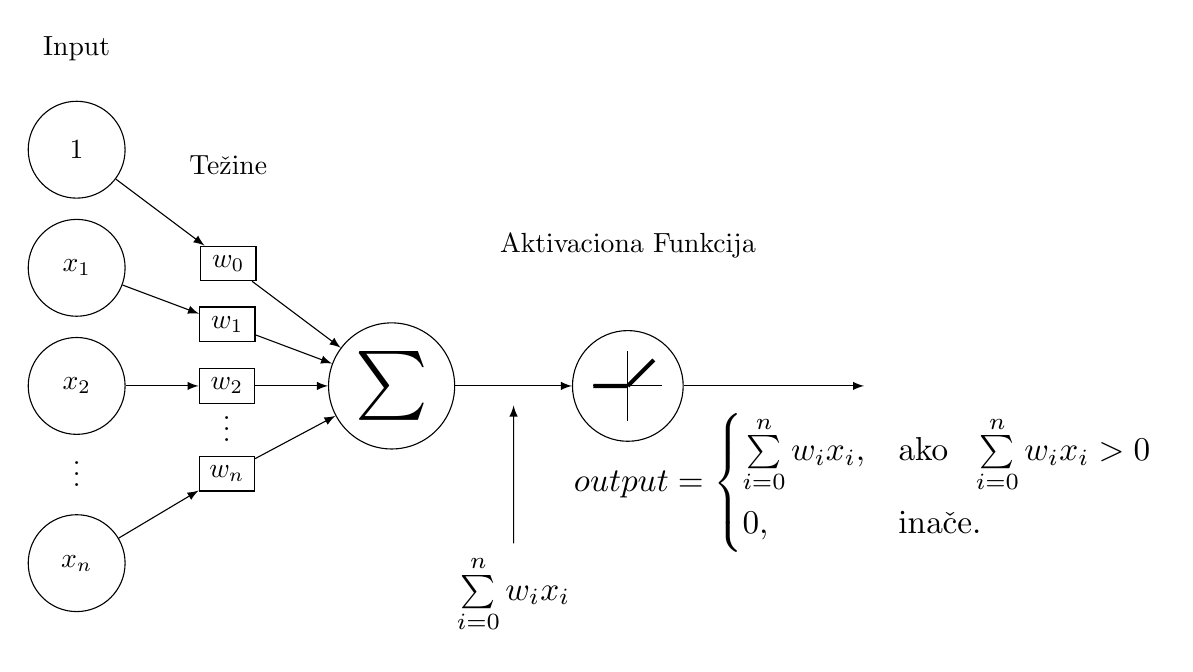
\begin{tikzpicture}[scale=1]
            
            % Draw input nodes
            \foreach \h [count=\hi ] in {$x_2$,$x_1$,$1$}{%
            \node[input] (f\hi) at (0,\hi*1.5cm-1.5 cm) {\h};
            }
            % Dot dot dot ... x_n
            \node[below=0.62cm] (idots) at (f1) {\vdots};
            \node[input, below=0.62cm] (last_input) at (idots) {$x_n$};
            % Draw summation node
            \node[functions] (sum) at (4,0) {\Huge$\sum$};
            % Draw edges from input nodes to summation node
            \foreach \h [count=\hi ] in {$w_2$,$w_1$,$w_0$}{%
            \path (f\hi) -- node[weights] (w\hi) {\h} (sum);
            \draw[->] (f\hi) -- (w\hi);
            \draw[->] (w\hi) -- (sum);
            }
         % Dot dot dot ... w_n
         \node[below=0.05cm] (wdots) at (w1) {\vdots};
         \node[weights, below=0.45cm] (last_weight) at (wdots) {$w_n$};
         % Add edges for last node and last weight etc
         \path[draw,->] (last_input) -- (last_weight);
         \path[draw,->] (last_weight) -- (sum);
         % Draw node for activation function
         \node[functions] (activation) at (7,0) {};
         % Place activation function in its node
         \begin{scope}[xshift=7cm,scale=1.25]
            \addaxes
            % flexible selection of activation function
            \relu
            %  \stepfunc
         \end{scope}
         % Connect sum to activation function
         \draw[->] (sum) -- (activation) node (sum_eq) [midway, below=2cm, scale=1.2] {$\sum\limits_{i=0}^n w_ix_i$} node (sum_activation_midway) [midway, below] {};
         \path[draw,->] (sum_eq) -- (sum_activation_midway);
         \draw[->] (activation) -- ++(3,0) node (perceptron_output) [below=0.2cm, scale=1.2] {$output = \begin{cases}\sum\limits_{i=0}^n w_ix_i, & \text{ako }\ \sum\limits_{i=0}^n w_ix_i > 0\\0, & \text{inače.}\end{cases}$};
         % Labels
         \node[above=1cm]  at (f3) {Input};
         \node[above=1cm] at (w3) {Težine};
         \node[above=1.5cm] at (activation) {Aktivaciona Funkcija};
      \end{tikzpicture}
      \caption{Grafički prikaz perceptrona}
      \label{fig:perceptron}
   \end{figure}
   
   \newpage
   \subsubsection*{Višeslojni Perceptron (MLP)}
   \textbf{MLP} je potpuno povezana veštačka neuronska mreža koja se sastoji od više 
   slojeva perceptrona, obično uključujući ulazni sloj, jedan ili više skrivenih slojeva i 
   izlazni sloj \cite{perceptron}.

   Za \textbf{MLP} sa \(L\) slojeva, ulaz u mrežu je \(\mathbf{x} \in \mathbb{R}^n\). 
   Izlaz svakog sloja \(l\) se računa kao:
   \[
   \mathbf{h}^{(l)} = f(\mathbf{W}^{(l)} \mathbf{h}^{(l-1)} + \mathbf{b}^{(l)})
   \]
   gde:
   \vspace{-0.5cm}
   \begin{itemize}
      \item \(\mathbf{h}^{(0)} = \mathbf{x}\) je ulazni vektor,
      \item\(\mathbf{W}^{(l)}\) i \(\mathbf{b}^{(l)}\) su matrica težina i vektor pomeraja za sloj \(l\),
      \item \(f\) je aktivaciona funkcija (obično \textit{ReLU}, \textit{sigmoid} ili \textit{tanh}).
   \end{itemize}

   Finalni sloj često koristi \textit{softmax} funkciju za klasifikacione zadatke, koja pretvara 
   izlaz u distribuciju verovatnoća za date klase:

   \[
   \text{softmax}(\mathbf{z})_i = \frac{e^{z_i}}{\sum_{j=1}^P e^{z_j}}
   \]

   gde je \(\mathbf{z}\) ulaz u softmax funkciju, a \(P\) je broj klasa.
   \vspace{0.5cm}

   \begin{figure}[h!]
      % NEURAL NETWORK with coefficients, uniform arrows
      \newcommand\setAngles[3]{
         \pgfmathanglebetweenpoints{\pgfpointanchor{#2}{center}}{\pgfpointanchor{#1}{center}}
         \pgfmathsetmacro\angmin{\pgfmathresult}
         \pgfmathanglebetweenpoints{\pgfpointanchor{#2}{center}}{\pgfpointanchor{#3}{center}}
         \pgfmathsetmacro\angmax{\pgfmathresult}
         \pgfmathsetmacro\dang{\angmax-\angmin}
         \pgfmathsetmacro\dang{\dang<0?\dang+360:\dang}
         }
      \centering
      \begin{tikzpicture}[x=3.2cm,y=1cm]
      \message{^^JNeural network with uniform arrows}
      \readlist\Nnod{4,5,3} % array of number of nodes per layer
      
      \foreachitem \N \in \Nnod{ % loop over layers
         \def\lay{\Ncnt} % alias of index of current layer
         \pgfmathsetmacro\prev{int(\Ncnt-1)} % number of previous layer
         \message{^^J Layer \lay, N=\N, prev=\prev ->}
         
         % NODES
         \foreach \i [evaluate={\y=\N/2-\i; \x=\lay; \n=\nstyle; \notation=(\lay==1)?"x":((\lay==\Nnodlen)?"y":"h");}] in {1,...,\N}{ % loop over nodes
               \message{N\lay-\i, }
               \node[node \n] (N\lay-\i) at (\x,\y) {$\notation_\i^{(\prev)}$};
            }    
         % CONNECTIONS
         \foreach \i in {1,...,\N}{ % loop over nodes
            \ifnum\lay>1 % connect to previous layer
            \setAngles{N\prev-1}{N\lay-\i}{N\prev-\Nnod[\prev]} % angles in current node
            %\draw[red,thick] (N\lay-\i)++(\angmin:0.2) --++ (\angmin:-0.5) node[right,scale=0.5] {\dang};
            %\draw[blue,thick] (N\lay-\i)++(\angmax:0.2) --++ (\angmax:-0.5) node[right,scale=0.5] {\angmin, \angmax};
            \foreach \j [evaluate={\ang=\angmin+\dang*(\j-1)/(\Nnod[\prev]-1);}] %-180+(\angmax-\angmin)*\j/\Nnod[\prev]
                        in {1,...,\Nnod[\prev]}{ % loop over nodes in previous layer
               \setAngles{N\lay-1}{N\prev-\j}{N\lay-\N} % angles out from previous node
               \pgfmathsetmacro\angout{\angmin+(\dang-360)*(\i-1)/(\N-1)} % number of previous layer
               %\draw[connect arrow,white,line width=1.1] (N\prev-\j.{\angout}) -- (N\lay-\i.{\ang});
               \draw[connect arrow] (N\prev-\j.{\angout}) -- (N\lay-\i.{\ang}); % connect arrows uniformly
            }
            \fi % else: nothing to connect first layer
         }
      }
      
      % LABELS
      \node[above=5,align=center,mygreen!60!black] at (N1-1.90) {input\\[-0.2em]sloj};
      \node[above=1,align=center,myblue!60!black] at (N2-1.90) {skriveni slojevi};
      \node[above=8,align=center,myred!60!black] at (N\Nnodlen-1.90) {output\\[-0.2em]sloj};
      
      \end{tikzpicture}
      \caption{Grafički prikaz \textbf{MLP}-a sa 4 ulazna, 5 skrivenih i 3 izlazna čvora}
      \label{fig:mlp}
   \end{figure}

   \newpage
   \section{Transformeri}
   \subsection{Istorija i razvoj}
   Model \textbf{Transformera}, predstavljen u seminalnom radu \textit{"Attention is All You Need"} \cite{attentionneed} od Vaswani-ja i saradnika 2017. godine, 
   označio je značajan napredak u oblasti obrade prirodnog jezika (\textbf{NLP}). 
   Pre toga, modeli kao što su Rekurentne Neuronske Mreže (\textbf{RNN}) \cite{rnn} i 
   \textit{Long Short-Term Memory} Mreže (\textbf{LSTM}) \cite{lstm} bili su dominantne arhitekture za 
   \textit{sequence-to-sequence} zadatke. Međutim, ovi modeli su imali ograničenja, 
   posebno sa udaljenim zavisnostima i paralelizacijom.

   Transformeri su revolucionisali \textbf{NLP} uvođenjem nove arhitekture koja se u potpunosti zasniva na 
   \textbf{\textit{self-attention}} mehanizmu, eliminišući potrebu za rekurentnim slojevima. 
   Ova inovacija je omogućila efikasnije treniranje i sposobnost da se bolje modeluju veze između 
   udaljenih reči u sekvenci. Uvođenje transformera dovelo je do dramatičnog poboljšanja performansi 
   na različitim \textbf{NLP} zadacima, kao što su mašinsko prevođenje, sažimanje teksta i odgovaranje na pitanja.

   Njihov uspeh brzo je postao evidentan razvojem moćnih modela koji su ih koristili kao osnovu. 
   Jedna od prvih značajnih primena bila je u mašinskom prevođenju, gde je transformer 
   nadmašio prethodne najbolje modele na referentnim skupovima podataka. 
   Ovaj uspeh je dodatno pojačan stvaranjem modela kao što su \textbf{BERT} 
   \textit{(Bidirectional Encoder Representations from Transformers)} \cite{bert} i \textbf{GPT} 
   \textit{(Generative Pre-trained Transformer)} \cite{gpt2}, koji su postavili nove standarde za 
   različite \textbf{NLP} zadatke.

   \subsection{Motivacija za transformer arhitekturu}

   Pre pojave transformera, Rekurentne Neuronske Mreže (\textbf{RNN}) i 
   \textit{Long Short-Term Memory} Mreže (\textbf{LSTM}) bile su primarni 
   modeli korišćeni za zadatke sa sekvencijalnim podacima u \textbf{NLP}-u. 
   Iako su ovi modeli bili donekle efikasni, imali su ograničenja naročito kod zadataka koji 
   uključuju udaljene zavisnosti \cite{trans_motivation}.

   \subsubsection{Rekurentne Neuronske Mreže (RNN)}
   \textbf{RNN}-ovi obrađuju sekvence podataka održavanjem skrivenog stanja (eng. \textbf{\textit{hidden state}}) 
   koje čuva informacije o prethodnim elementima u sekvenci (\textit{Slika 8}). 
   Skriveno stanje u vremenskom koraku \( t \), označeno kao \( h_t \), se računa kao:

   \[ h_t = f(W_{hh} h_{t-1} + W_{xh} x_t + b_h) \]

   gde:
   \begin{itemize}
      \vspace{-0.5cm}
      \setlength\itemsep{0.2em} % Set the vertical space between items
      \item \( x_t \) je ulaz u vremenskom koraku \( t \),
      \item \( W_{hh} \) i \( W_{xh} \) su matrice težina,
      \item \( b_h \) je pomeraj,
      \item \( f \) je aktivaciona funkcija (npr. \(\tanh\)).
   \end{itemize}

   \textbf{RNN}-ovi pate od problema nestajućih i eksplodirajućih gradijenata (eng. \textbf{\textit{vanishing and exploding gradients}}), 
   što otežava efikasno učenje udaljenih zavisnosti. Gradijenti \textit{loss} funkcije ili opadaju ili rastu 
   eksponencijalno tokom propagacije unazad (\textbf{\textit{backpropagation}}), što dovodi 
   do slabog učenja udaljenih zavisnosti \cite{rnn_downsides}.
   
   \begin{figure}[h!]
      \centering
      \vspace{1.5cm} % Add vertical space
      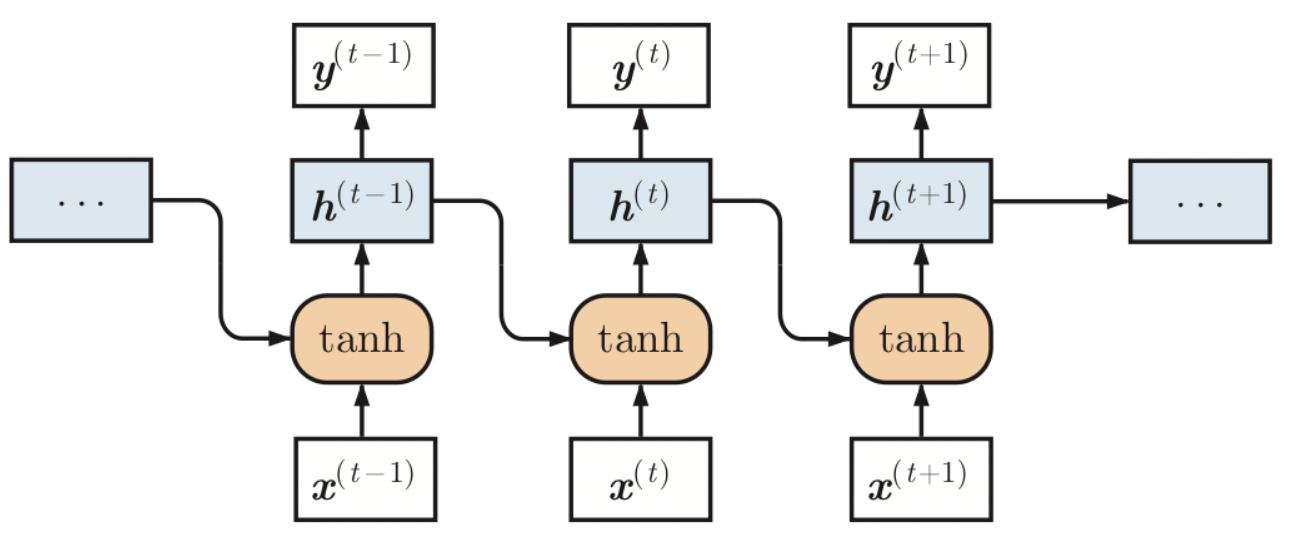
\includegraphics[width=0.8\textwidth]{rnn.png}
      \caption{Prikaz rekurentne neuronske mreže \cite{rnn_pic}}
      \label{fig:rnn}
   \end{figure}

   \subsubsection{Long Short-Term Memory Mreže (LSTM)}
   \textbf{LSTM}-ovi su uvedeni da bi rešili neka od ograničenja \textbf{RNN}-ova \cite{lstms_explained0}. 
   Uključuju memorijske ćelije i mehanizme za kontrolu protoka informacija, 
   omogućavajući im da efikasnije modeluju udaljene zavisnosti. Ključne komponente \textbf{LSTM}-a su ćelije 
   koje se sastoje od: ulazne kapije (\( i_t \)), zaboravne kapije (\( f_t \)), izlazne kapije (\( o_t \)) i 
   stanja ćelije (\( c_t \)), detaljnije na \textit{Slici 9}. Stanje ćelije se ažurira kao:

   \[ c_t = f_t \odot c_{t-1} + i_t \odot \tilde{c}_t \]

   gde je $\odot$ Adamarov proizvod, a \( \tilde{c}_t \) kandidat za stanje ćelije, obično računat kao:

   \[ \tilde{c}_t = \tanh(W_{xc} x_t + W_{hc} h_{t-1} + b_c). \]

   Iako \textbf{LSTM}-ovi ublažavaju neke probleme \textbf{RNN}-ova, i dalje se suočavaju sa 
   izazovima u paralelizaciji i računskoj efikasnosti. Sekvencijalna priroda njihove
   obrade znači da ne mogu efikasno koristiti paralelno izračunavanje, što ograničava njihovu 
   skalabilnost.

   \begin{figure}[h!]
      \centering
      \vspace{1.5cm} % Add vertical space
      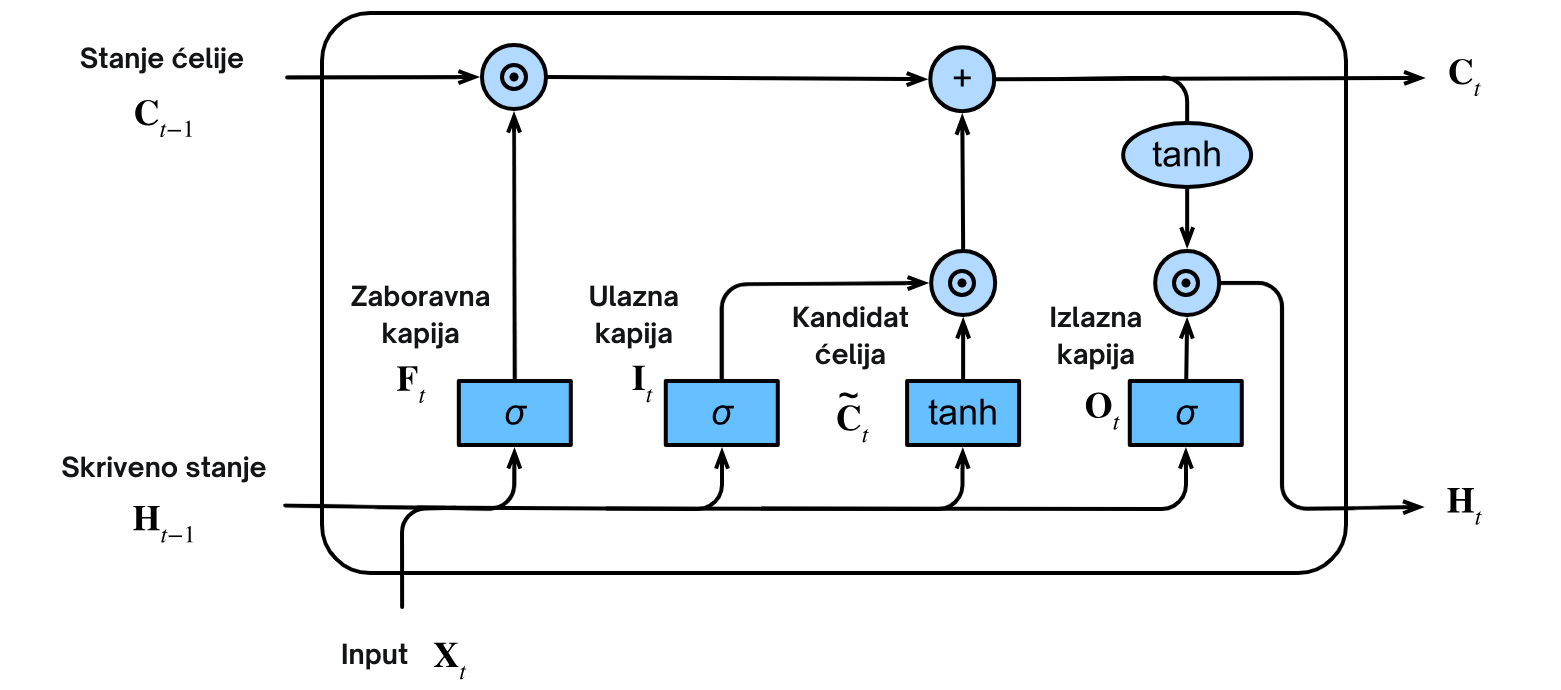
\includegraphics[width=1\textwidth]{lstm.png}
      \caption{Prikaz arhitekture \textbf{LSTM} modela \cite{lstms_explained}}
      \label{fig:lstm}
   \end{figure}

   \subsubsection{Prednost transformera}
   Transformeri rešavaju ova ograničenja koristeći potpuno drugačiji mehanizam poznat kao 
   \textbf{\textit{self-attention}} mehanizam, koji omogućava efikasnu paralelizaciju i poboljšano 
   rukovanje udaljenim zavisnostima. \textit{Self-attention} mehanizam računa \textit{attention} 
   rezultate za svaki par elemenata u ulaznoj sekvenci, modelujući zavisnosti bez obzira na njihovu
   udaljenost. Ovaj mehanizam omogućava transformer modelu da procesira sve elemente 
   sekve-nce istovremeno, omogućavajući efikasnu paralelizaciju. 
   
   Pored toga, korišćenje \textbf{\textit{multi-head attention}} mehanizma dodatno poboljš-ava 
   sposobnost mreže da modeluje različite aspekte odnosa između elemenata u sekvenci.

   Korišćenjem \textit{self-attention} i \textit{multi-head attention} mehanizama, transformeri 
   prevazilaze ograničenja \textbf{RNN}-ova i \textbf{LSTM}-ova, pružajući značajna 
   pobolj-šanja u performansama i efikasnosti za širok spektar \textbf{NLP} zadataka \cite{attentionneed}.

   \subsection{Arhitektura transformera}

   Arhitektura transformera sastoji se od dva glavna dela (\textit{Slika 10}):
   \begin{itemize}
      \item \textbf{Enkoder} 
      \item \textbf{Dekoder}
   \end{itemize}
   Obe komponente su dizajnirane da rade zajedno u zadacima poput mašinskog prevođenja, 
   gde enkoder obrađuje ulaznu sekvencu, a dekoder generiše odgovarajuću izlaznu sekvencu. 

   \newpage
   
   \begin{figure}[h!]
      \centering
      \vspace{-1cm} % Add vertical space
      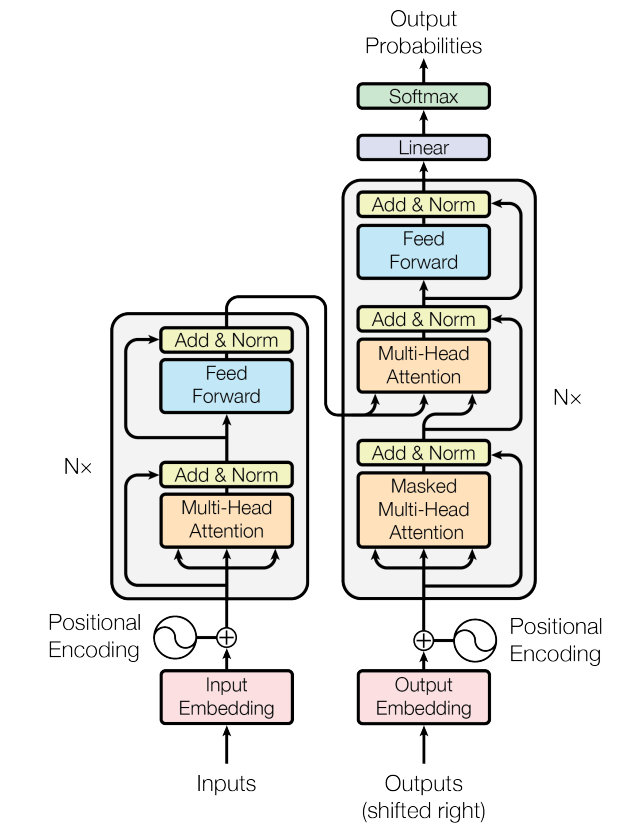
\includegraphics[width=0.7\textwidth]{transformer.png}
      \caption{Transformer arhitektura \cite{attentionneed}}
      \label{fig:transformer}
   \end{figure}

   \subsubsection{Enkoder}
   Enkoder je odgovoran za obradu ulazne sekvence i ekstrahovanje njenih reprezentacija \cite{trans_exp}.

   \subsubsection*{Input Embedding}

   Pre nego što se bilo koja ulazna sekvenca može obraditi od strane transformera, 
   ona mora biti konvertovana u neprekidnu vektorsku reprezentaciju. 
   Ovo se postiže kroz \textit{embedding} sloj , 
   koji mapira svaki token\footnote{Token predstavlja osnovnu jedinicu 
   informacije, koja može biti reč, deo reči ili simbol, a koristi se kao 
   ulazni podatak u enkoder.} ulazne sekvence u vektor fiksne veličine, 
   označen sa \( d_{\text{model}} \), kao što je prikazano na \textit{Slici 11}.

   \newpage
   Za datu ulaznu sekvencu tokena \(\{x_1, x_2, \dots, x_\text{seq}\}\), 
   svaki token \(x_i\) se mapira u \textit{embedding} vektor \(E(x_i)\) 
   veličine \( d_{\text{model}} \). Ova mapiranja se uče tokom procesa treniranja 
   i obično se predstavljaju kao:
   \[
   E: \{x_1, x_2, \dots, x_\text{seq}\} \rightarrow \mathbb{R}^{d_{\text{model}}}.
   \]

   Tako se ulazna sekvenca \(\{x_1, x_2, \dots, x_\text{seq}\}\) transformiše u 
   \textit{embedding} matricu \(X \in \mathbb{R}^{\text{seq} \times d_{\text{model}}}\), gde svaki 
   red odgovara embedovanju određenog tokena u sekvenci:

   \[
   X = \begin{bmatrix}
   E(x_1) \\
   E(x_2) \\
   \vdots \\
   E(x_\text{seq})
   \end{bmatrix}
   \]

   \begin{figure}[h!]
      % \centering
      \hspace{-2cm} % Add horizontal space
      % \vspace{-1cm} % Add vertical space
      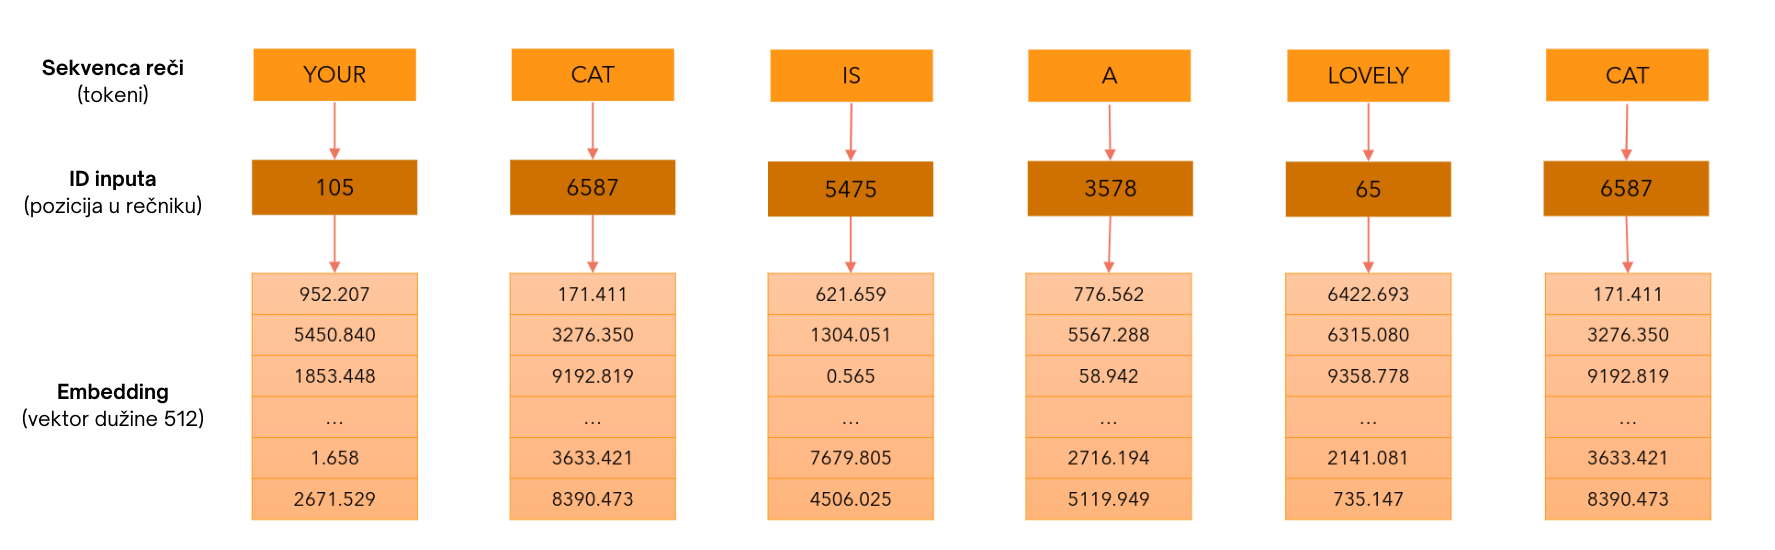
\includegraphics[width=1.3\textwidth]{token.png}
      \caption{Embedovanje tokena u vektorski prostor \cite{transformer}}
      \label{fig:token_embedding}
   \end{figure}

   \newpage

   \subsubsection*{Poziciono enkodovanje (eng. positional encoding)}
   Da bi model bio sposoban da prepozna redosled tokena u sekvenci, pozicioni vektori 
   se dodaju na \textit{embedding} vektore. Ovi vektori unose informaciju o poziciji 
   svakog tokena, omogućavajući modelu da razlikuje tokene na osnovu njihove pozicije 
   u sekvenci \cite{attentionneed}.

   Pozicioni vektori mogu biti naučeni, kao što se uče i \textit{embedding} vektori, ili mogu biti fiksni, 
   zasnovani na unapred definisanim funkcijama. Autori transformera odlučili su da 
   koriste fiksne vektore, koji su davali gotovo iste rezultate kao i naučeni, 
   dok su pritom bili jednostavniji i lakši za interpretaciju.

   Fiksni pozicioni vektori (\textit{Slika 12}) za svaku poziciju \( pos \) u sekvenci definisani su kao:
   \[
      PE_{(pos, 2i)} = \sin\left(\frac{pos}{10000^{2i/d_{\text{model}}}}\right)
   \]
   \vspace{-0.5cm}
   \[
         PE_{(pos, 2i+1)} = \cos\left(\frac{pos}{10000^{2i/d_{\text{model}}}}\right)
   \]
         
   gde:
   \begin{itemize}
      \vspace{-0.5cm}
      \item \( pos \) je pozicija tokena u sekvenci.
      \item \( i \) je indeks dimenzije (od 0 do \( d_{\text{model}}/2 - 1 \)).
   \end{itemize}

   \begin{figure}[h!]
      % \centering
      \hspace{-2cm} % Add horizontal space
      % \vspace{-1cm} % Add vertical space
      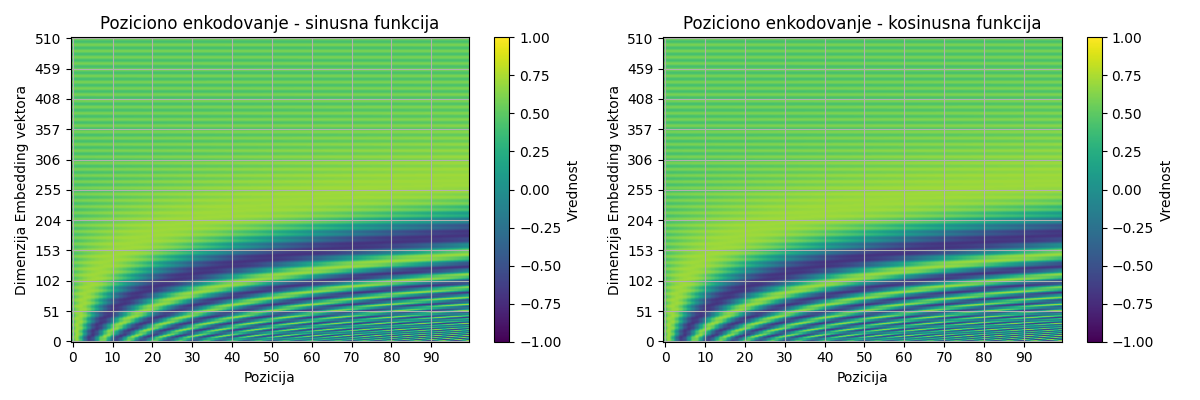
\includegraphics[width=1.3\textwidth]{pos_encoding.png}
      \caption{Grafik pozicionog enkodovanja za sinusnu i kosinusnu funkciju}
      \label{fig:pos_encoding}
   \end{figure}

   Korišćenje \textbf{sinusnih} i \textbf{kosinusnih} funkcija osigurava da su pozicioni vektori
   neprekidni i glatki, što pomaže u očuvanju relativnih pozicionih informacija. 
   
   Pored toga, ove funkcije imaju periodične osobine koje omogućavaju modelu da 
   generalizuje na sekvence različitih dužina, jer slične pozicije proizvode slične 
   pozicione vektore čak i u dugačkim sekvencama.

   Ovi pozicioni vektori se dodaju na \textit{embedding} vektore:

   \[
   X' = X + PE
   \]

   gde je \(X'\) konačni ulaz u enkoder, koji kombinuje \textit{embedding} vektor 
   sa pozicionim vektorom. Ova kombinacija omogućava transformeru da 
   iskoristi i sadržaj i redosled tokena u sekvenci, što omogućava efikasnije 
   učenje i predikciju \cite{attentionneed}.

   \subsubsection*{Self-Attention mehanizam}
   \textbf{\textit{Self-attention} mehanizam} \cite{attentionneed} omogućava modelu da odredi značaj nekog 
   tokena u ulaznoj sekvenci u odnosu na ostale ulazne tokene. 
   Na taj način model može da modeluje zavisnosti između tokena, bez obzira na 
   njihovu udaljenost u sekvenci, što predstavlja značajnu prednost u odnosu na 
   tradicionalne rekurentne neuronske mreže (\textbf{RNN}).
 
   Težine, odnosno \textit{attention} vrednosti, predstavljaju koliko fokusa model treba 
   da usmeri na ostale tokene prilikom obrade određenog tokena \cite{trans_exp}. 
   Ove vrednosti se izračunavaju koristeći tri ključne komponente izvedene 
   iz ulaznih \textit{embedding} vektora:

   \begin{itemize}
      \item \textbf{Upit (Q, Query):} Predstavlja token koji trenutno obrađujemo,
      \item \textbf{Ključ (K, Key):} Predstavlja tokene u sekvenci sa kojima 
      se upoređuje trenutni token,
      \item \textbf{Vrednost (V, Value):} Predstavlja stvarne informacije tokena koje 
      će se koristiti kasnije u množenju.
  \end{itemize}
  
  \newpage

  Za svaki token u sekvenci, računamo vektore \textbf{Upita}, \textbf{Ključa} i \textbf{Vrednosti}:
   \vspace{-0.2cm} % Add vertical space
  \[
  Q = XW^Q, \quad K = XW^K, \quad V = XW^V
  \]
  \vspace{-0.7cm} % Add vertical space
  gde su:
  \begin{itemize}
   \vspace{0.2cm} % Add vertical space
      \item \( X \) matrica ulaznih \textit{embedding} vektora 
      dimenzija \( \text{seq} \times d_{\text{model}} \),
      \item \( W^Q, W^K, W^V \) matrice težina dimenzija 
      \( d_{\text{model}} \times d_k \), \( d_{\text{model}} \times d_k \), 
      i \( d_{\text{model}} \times d_v \),
      \item \( d_k \) i \( d_v \) dimenzije vektora \textbf{Upita}/\textbf{Ključa} i \textbf{Vrednosti}, 
      često su \\ \( d_k = d_v = d_{\text{model}}/h \), gde je \( h \) 
      broj \textit{self-attention} glava (o čemu će biti reči u narednom odeljku).
  \end{itemize}
  
  \textit{Attention} vrednosti za svaki par tokena se izračunavaju kao skalarni proizvod 
  \textbf{Upita} trenutnog tokena sa \textbf{Ključem} drugog tokena, 
  skaliran kvadratnim korenom dimenzije \( d_k \), nakon čega sledi \textit{softmax} 
  funkcija koja normalizuje rezultate (\textit{Slika 13}):
  
  \vspace{-0.7cm} % Add vertical space
  \[
  \text{Attention}(Q, K, V) = \text{softmax}\left(\frac{QK^T}{\sqrt{d_k}}\right)V.
  \]
  \vspace{-0.7cm} % Add vertical space

  Skaliranje sa \( \sqrt{d_k} \) sprečava da skalarni proizvod postane prevelik, 
  što bi moglo dovesti do vrlo malih gradijenata i sporog treniranja.

   \begin{figure}[h!]
   \centering
   % \vspace{-1cm} % Add vertical space
   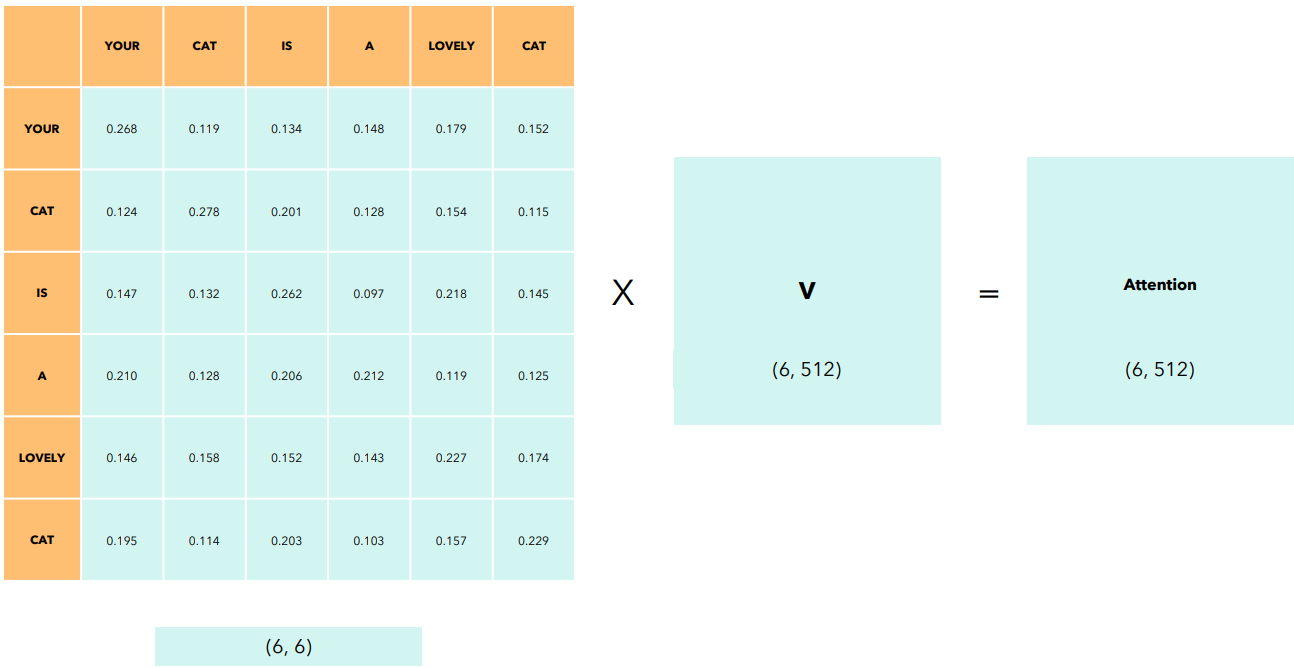
\includegraphics[width=1.1\textwidth]{self_attention.png}
   \caption{Prikaz \textit{self-attention} mehanizma \cite{transformer}}
   \label{fig:self_attention}
   \end{figure}

   \subsubsection*{Multi-Head Attention}
   Kako bi se modelovali različiti tipovi odnosa između tokena, Transformer koristi 
   \textit{multi-head attention} mehanizam. Umesto da se izračuna jedan skup vektora 
   \textbf{Upita}, \textbf{Ključa} i \textbf{Vrednosti}, ulaz se projektuje u više 
   podprostora (glava), od kojih svaka ima svoj skup matrica težina (\textit{Slika 14}). Ovo omogućava modelu da 
   nauči različite aspekte odnosa između tokena \cite{trans_exp}.

   Za svaku glavu \( i \):

   \[
   Q_i = XW_i^Q, \quad K_i = XW_i^K, \quad V_i = XW_i^V.
   \]

   Svaka glava izračunava svoj izlaz operatora pažnje:

   \[
   \text{head}_i = \text{Attention}(Q_i, K_i, V_i).
   \]

   Izlazi svih glava se zatim konkateniraju i projektuju nazad na originalnu 
   dimenziju \( d_{\text{model}} \):

   \[
   \text{MultiHead}(Q, K, V) = \text{Concat}(\text{head}_1, \dots, \text{head}_h)W^O
   \]

   gde je \( W^O \) matrica težina dimenzija \( hd_v \times d_{\text{model}} \) (\textit{Slika 15}).

   \begin{figure}[h!]
      \centering
      % \hspace{-2cm} % Add horizontal space
      \vspace{0.5cm} % Add vertical space
      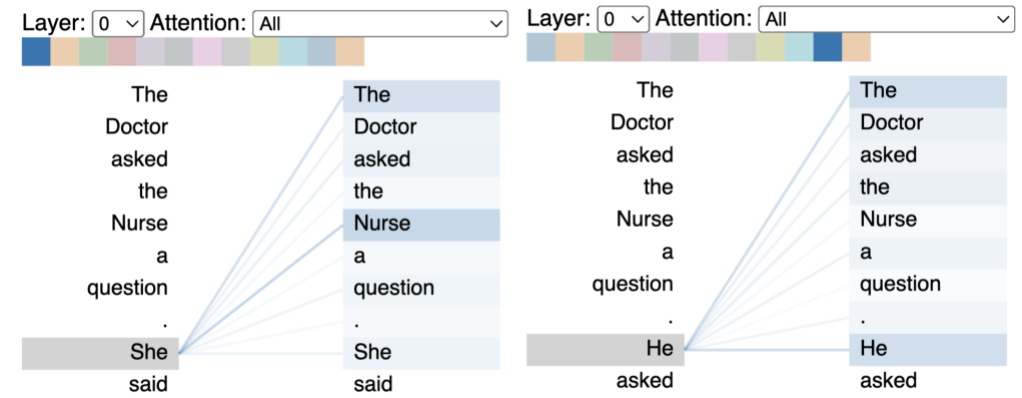
\includegraphics[width=1\textwidth]{attention_head.png}
      \caption{Vizuelizacija jedne glave \textit{multi-head attention} mehanizma \cite{attention_head}}
      \label{fig:attention_head}
   \end{figure}


   \newpage
   \begin{figure}[h!]
      % \centering
      \hspace{-2cm} % Add horizontal space
      \vspace{-0.5cm} % Add vertical space
      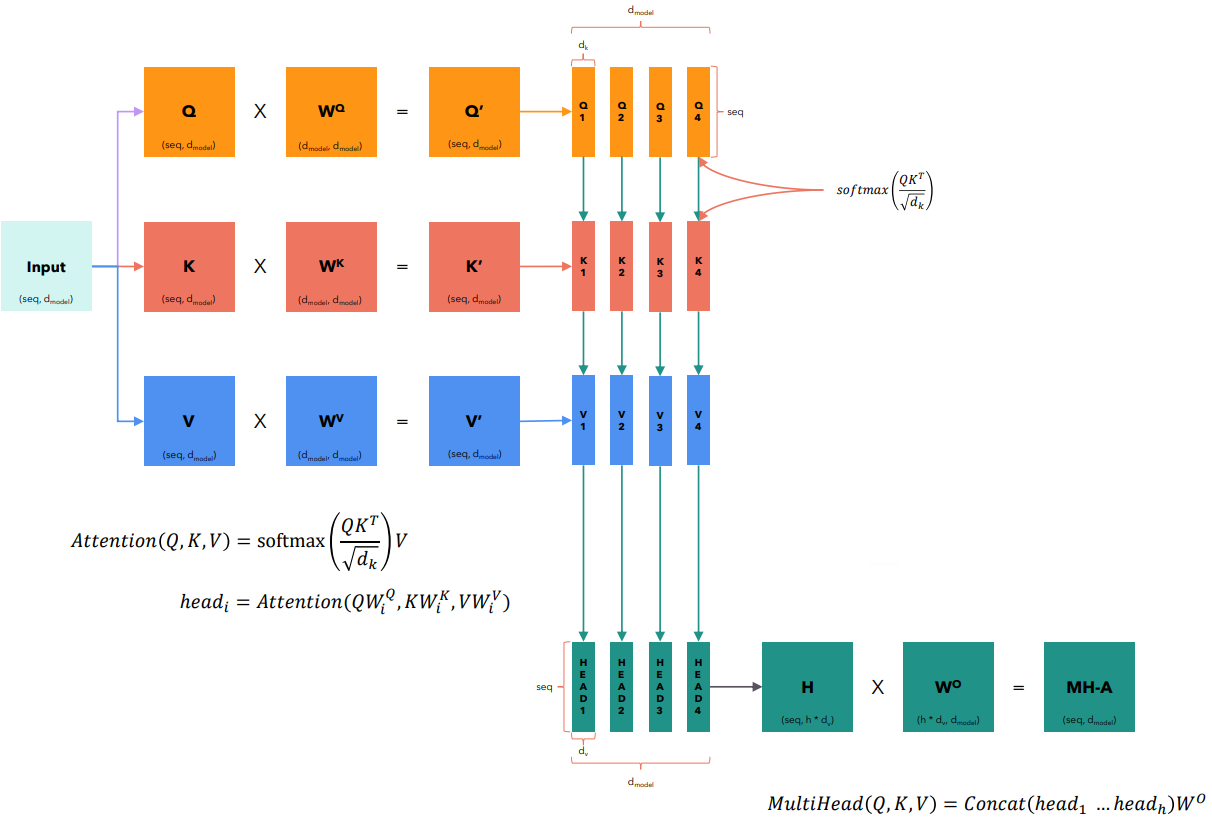
\includegraphics[width=1.3\textwidth]{mha.png}
      \caption{Grafik \textit{multi-head attention} mehanizma \cite{transformer}}
      \label{fig:mha}
   \end{figure}

   \subsubsection*{Intuicija i Uticaj}

   Notacija $K$, $Q$ i $V$ inspirisana je konceptima ključa (key), upita (query) i 
   vrednosti (value) iz sistema baza podataka (\textit{Slika 16}).

   \textit{Self-attention} mehanizam omogućava transformeru da razume kontekst reči u sekvenci 
   gledajući druge reči u sekvenci, bez obzira na njihov položaj \cite{trans_exp}. 
   Ovo je ključno za modelovanje udaljenih zavisnosti, čineći transformere posebno efikasnim u 
   zadacima kao što su jezičko modelovanje, prevođenje i, kao što je to slučaj kod 
   Vision Transformera, klasifikacija slika.

   \newpage
   \begin{figure}[h!]
      \centering
      \vspace{-1cm} % Add vertical space
      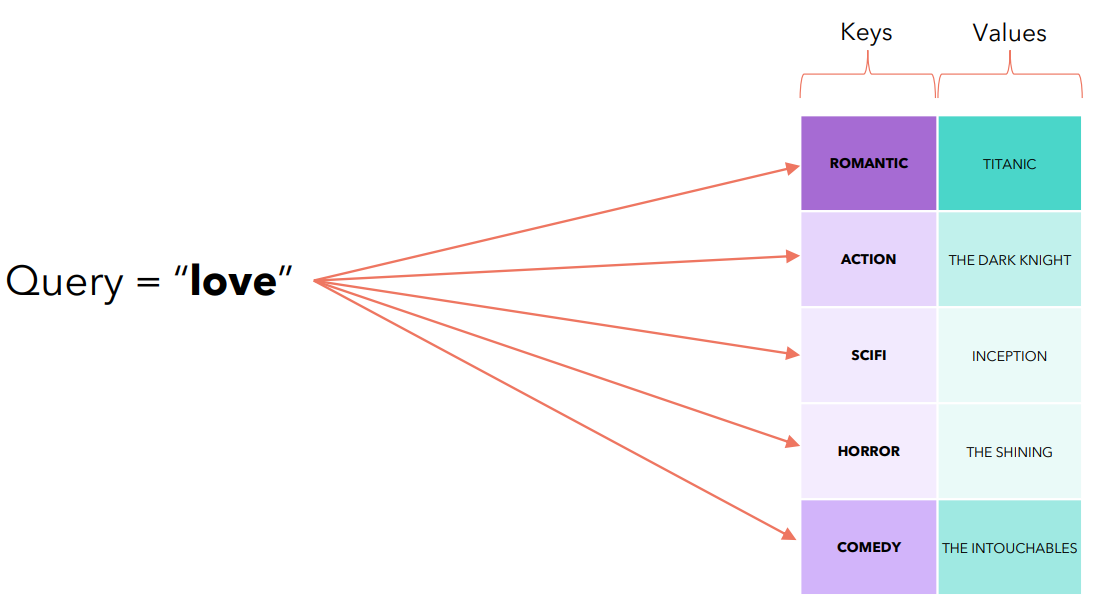
\includegraphics[width=0.9\textwidth]{dict.png}
      \caption{Koncepti ključa, upita i vrednosti dolaze iz baza podataka \cite{transformer}}
      \label{fig:trans_inspiration}
   \end{figure}

   \subsubsection*{Rezidualne Konekcije i Normalizacija Slojeva}

   Rezidualne konekcije i normalizacija slojeva su ključne tehnike koje poboljšavaju 
   stabilnost i performanse tokom obuke.

   Rezidualne konekcije (\textit{skip} konekcije) omogućavaju da se ulaz sloja direktno 
   doda njegovom izlazu, što pomaže u rešavanju problema nestajanja gradijenta. Ovo 
   olakšava obuku dubljih mreža omogućavajući da gradijenti lakše teku kroz mrežu.

   Formalno:
   \[
   \text{Output} = \text{Layer}(x) + x
   \]
   gde:
   \begin{itemize}
      \vspace{-0.5cm}
      \item \( x \) je ulaz u sloj,
      \item \( \text{Layer}(x) \) je izlaz transformacije sloja.
   \end{itemize}

   Ovo dodavanje rezidualne konekcije omogućava modelu da očuva originalne informacije.
   
   Normalizacija slojeva stabilizuje i ubrzava obuku normalizovanjem aktivacija duž 
   svih dimenzija svakog uzorka ponaosob. Razlikuje se od \textit{batch} normalizacije po 
   tome što normalizuje svaki pojedinačni uzorak umesto duž cele serije \cite{batch_vs_layer}.

   Formalno:
   \[
   \text{LayerNorm}(x) = \frac{x - \mu}{\sigma} \cdot \gamma + \beta
   \]
   gde:
   \begin{itemize}
      \vspace{-0.5cm}
      \setlength\itemsep{0.2em} % Set the vertical space between items
      \item \( x \) je ulazni vektor,
      \item \( \mu \) i \( \sigma \) su srednja vrednost i standardna devijacija \( x \),
      \item \( \gamma \) i \( \beta \) su parametri za skaliranje i pomeranje koji se uče.
   \end{itemize}

   U transformeru, normalizacija slojeva se primenjuje nakon rezidualne konekcije:
   \[
   \text{Output} = \text{LayerNorm}(\text{Layer}(x) + x).
   \]  
   Ove tehnike osiguravaju da model efikasno trenira, održava stabilne gradijente i 
   omogućava korišćenje dubljih neuronskih mreža bez značajnih problema sa performansama.

   \subsubsection{Dekoder}
   Dekoder je odgovoran za generisanje izlazne sekvence, poput prevođenja rečenice s jednog jezika 
   na drugi. Deli sličnosti sa enkoderom, ali uvodi dodatne mehanizme za obradu sekvencijalnih 
   podataka i za obraćanje pažnje na izlaz enkodera.

   Dekoder ima tri glavne komponente:
   \begin{itemize}
      \item Maskirani \textit{Self-Attention} Mehanizam
      \item \textit{Enkoder-Dekoder Attention} Mehanizam
      \item \textit{Feed-Forward} Neuronska Mreža (\textbf{FFN}, ranije \textbf{MLP})
   \end{itemize}

   Ove komponente su kombinovane sa rezidualnim konekcijama i 
   normalizacijom slojeva, slično kao kod enkodera \cite{trans_exp}.

   \subsubsection*{Maskirani Self-Attention Mehanizam}
   \textit{Self-attention} mehanizam u dekoderu je sličan onom u enkoderu, ali sa 
   ključnom razlikom: \textbf{maskiranjem} (\textit{Slika 17}). Pri generisanju izlazne sekvence, 
   svaka pozicija može da se odnosi samo na prethodne pozicije, ne i na buduće. 
   Ovo sprečava dekoder da "vara" gledajući unapred u tokene koji još nisu generisani.

   \textit{Attention} težine se računaju kao:
   \[
   \text{Attention}(Q, K, V) = \text{softmax}\left(\frac{QK^T}{\sqrt{d_k}} + M\right)V
   \]
   \vspace{-0.7cm}
   gde:
   \begin{itemize}
      \item \( Q \), \( K \), i \( V \) su matrice upita, ključeva i vrednosti,
      \item \( d_k \) je dimenzija ključeva,
      \item \( M \) je matrica maske koja postavlja \textit{attention} težine na
      $-\infty$ za \\ nedozvoljene pozicije (one koje ne bi trebalo da budu obrađene).
   \end{itemize}

   \begin{figure}[h!]
      \centering
      % \hspace{-2cm} % Add horizontal space
      % \vspace{-0.5cm} % Add vertical space
      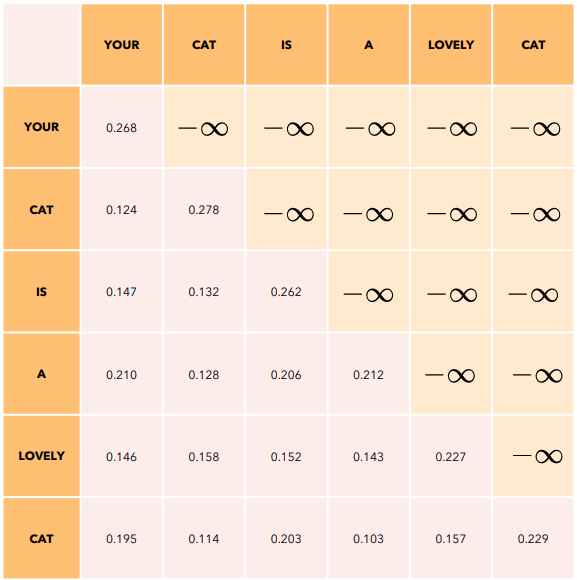
\includegraphics[width=0.6\textwidth]{masked_attention.png}
      \caption{Izgled $\frac{QK^T}{\sqrt{d_k}} + M$ matrice pre primene \textit{softmax} funkcije \cite{transformer}}
      \label{fig:masked_attention}
   \end{figure}

   \subsubsection*{Enkoder-Dekoder Attention}

   Nakon računanja maskiranog \textit{self-attention} mehanizma, dekoder obraća pažnju na 
   izlaz enkodera koristeći standardni \textit{attention} mehanizam. Ovo omogućava dekoderu da 
   se fokusira na relevantne delove ulazne sekvence dok generiše izlaz.

   \textit{Attention} mehanizam ovde se može opisati kao:
   \[
   \text{Attention}(Q, K, V) = \text{softmax}\left(\frac{QK^T}{\sqrt{d_k}}\right)V
   \]
   U ovom slučaju, \( Q \) dolazi iz prethodnog sloja dekodera, dok \( K \) i \( V \) 
   dolaze iz završnih slojeva enkodera.

   \subsubsection*{Feed-Forward Neuronska Mreža (FFN)}
   Nakon \textit{attention} slojeva, izlaz prolazi kroz \textbf{FFN} mrežu, 
   identičnu onoj koja se koristi u enkoderu. Ovaj modul se sastoji od dve 
   linearne transformacije sa \textit{ReLU} aktivacijom između njih \cite{attentionneed}:
   \[
   \text{FFN}(x) = \max(0, xW_1 + b_1)W_2 + b_2
   \]
   gde:
   \begin{itemize}
      \item \( W_1, W_2 \) su težinske matrice, a \( b_1, b_2 \) su pomeraji,
      \item \textit{ReLU} aktivacija uvodi nelinearnost.
   \end{itemize}

   \subsubsection*{Poslednji Linearni i Softmax Sloj}
   Nakon prolaska kroz više dekoderskih modula, konačni izlaz je sekvenca vektora, 
   jedan za svaku poziciju u ciljnoj sekvenci. Ovi vektori se transformišu 
   linearno i zatim prolaze kroz \textit{softmax} funkciju kako bi generisali verovatnoće 
   ciljnog vokabulara:
   \[
   P(\text{trenutna reč} \mid \text{prethodne reči}) = \text{softmax}(W_o \cdot h + b_o)
   \]
   \newpage
   gde:
   \begin{itemize}
      \vspace{-0.5cm}
      \setlength\itemsep{0.2em} % Set the vertical space between items
      \item \( W_o \) je težinska matrica izlaza,
      \item \( h \) je skriveno stanje iz poslednjeg dekoderskog sloja,
      \item \( b_o \) je pomeraj.
   \end{itemize}
   Dekoder generiše izlaznu sekvencu jedan po jedan token, vraćajući prethodno 
   generisane tokene u model sve dok cela sekvenca nije izgenerisana \cite{trans_exp}.

   \subsection{Generisanje}
   Tokom generisanja, transformer generiše predikcije za sekvencu na osnovu zadatog ulaza. 
   Ključni aspekt generisanja je da model obrađuje svaki token u sekvenci jedan po jedan, 
   koristeći prethodno generisane tokene za generisanje sledećeg. U ovom scenariju, 
   složenost je obično linearna u odnosu na dužinu sekvence \(n\).

   \begin{itemize}
       \item \textbf{Vremenska složenost:} \(O(n)\)
       \item \textbf{Opis:} Složenost proizlazi iz obrade svakog tokena u sekvenci pojedinačno.
   \end{itemize}

   \subsection{Trening}
   Transformer obrađuje celu sekvencu odjednom u toku treninga, koristeći paralelizam. 
   Sve pozicije se obrađuju simultano, što znači da je složenost konstantna u odnosu 
   na dužinu sekvence. Međutim, sam \textit{attention} mehanizam uključuje 
   izračunavanje međusobnih odnosa, što dovodi do kvadratne složenosti u odnosu 
   na dužinu sekvence.

   \begin{itemize}
      \item \textbf{Vremenska složenost:} \(O(1)\) za paralelnu obradu svakog tokena
      \item \textbf{Opis:} Trening koristi paralelnu obradu, ali ukupna složenost \textit{attention} 
      mehanizma je \(O(n^2)\) zbog međusobnih poređenja kroz dužinu sekvence.
   \end{itemize}

   \section{Vision Transformeri}
   \subsection{Istorija i razvoj}
   \textit{Vision} transformer (\textbf{ViT}) je predstavljen u radu 
   \textit{"An Image is Worth 16x16 Words: Transformers for Image Recognition at Scale"} \cite{vit} 
   autora Dosovitskiy i ostalih saradnika (2020). Primarna inovacija \textbf{ViT}-a je 
   prilagođavanje arhitekture transformera, prvobitno dizajnirane za \textbf{NLP}, 
   za rad sa vizuelnim podacima. Ova promena označava odstupanje od 
   tradicionalnih \textbf{CNN}-ova, koristeći prednosti \textit{self-attention} mehanizama za obradu slika.

   \subsection{Poređenje sa CNN-ovima}

   \begin{itemize}
      \item \textbf{Induktivna pretpostavka:}
      \begin{itemize}
         \item \textbf{CNN:} Ima jaku induktivnu pretpostavku zbog svojih konvolucionih filtara, 
         koji nameću lokalne prostorne hijerarhije, kao i \textit{pooling} slojeva
         koji omogućavaju translacionu invarijantnost. To znači 
         da \textbf{CNN}-ovi pretpostavljaju da su lokalne karakteristike (npr. ivice) važne, pa pošto
         filteri dele težine, mreža traga za tim obrascima unutar čitave slike.
         \item \textbf{ViT:} Nema ugrađenu ovu pretpostavku. Umesto toga, uči 
         odnose između svih delova slike putem \textit{self-attention} mehanizma, što mu 
         omogućava da modeluju globalne zavisnosti i interakcije između različitih delova slike \cite{vit}.
      \end{itemize}
      \item \textbf{Receptivno Polje:}
      \begin{itemize}
         \item \textbf{CNN:} Ima ograničeno receptivno polje, što znači da svaki filtar pokriva 
         samo malu, lokalizovanu oblast slike. Da bi se modelovao globalni kontekst, potrebni su 
         dublji slojevi ili veća receptivna polja, što povećava računsku složenost.
         \item \textbf{ViT:} Poredi svaki deo slike u odnosu na sve druge delove zahvaljujući
         \textit{self-attention} mehanizmu. Ovo znači da može modelovati udaljene zavisnosti od 
         samog početka, bez potrebe za dubokim ili složenijim arhitekturama \cite{vit}.
      \end{itemize}
   \end{itemize}

   \subsection{Prednosti i Nedostaci}
   \begin{itemize}
      \item \textbf{Prednosti:}
      \begin{itemize}
          \item \textbf{Globalni Kontekst:} Mogu da modeluju globalni kontekst 
          i odnose između svih delova slike od samog početka, zahvaljujući \textit{self-attention} 
          mehanizmu.
          \item \textbf{Fleksibilnost:} Nisu ograničeni na lokalnu obradu kao \textbf{CNN}-ovi i 
          mogu da nauče reprezentacije koje nisu ograničene strukturom konvolucionih filtara.
          \item \textbf{Skalabilnost:} Mogu se efikasno skalirati povećanjem podataka i računarskih 
          resursa. Vrlo lako se dotreniraju za specifične zadatke sa malim skupom podataka 
          koristeći prethodno obučene velike modele \cite{vit}.
      \end{itemize}
      \item \textbf{Nedostaci:}
      \begin{itemize}
         \item \textbf{Efikasnost Podataka:} Obično zahtevaju velike količine 
         podataka za efikasnu obuku. Nemaju istu induktivnu pretpostavku kao \textbf{CNN}-ovi, 
         što može dovesti do lošijih performansi sa ograničenim podacima \cite{vit}.
         \item \textbf{Računski Trošak:} Kvadratna složenost \textit{self-attention} mehanizma 
         može biti računski skupa, posebno za slike visoke rezolucije ili duge nizove tokena.
         \item \textbf{Složenost Obuke:} Obuka može biti izazovna i često zahteva pažljivo 
         podešavanje hiperparametara i velike računarske resurse.
      \end{itemize}
  \end{itemize}

  \newpage
  \subsection{Arhitektura Vision Transformera}
  Glavni delovi \textbf{ViT} \cite{vit} arhitekture (\textit{Slika 18}) su:
   \begin{itemize}
         \item \textbf{Tokenizacija slike}
         \item \textbf{Poziciono enkodovanje}
         \item \textbf{Transformer Enkoder}
         \item \textbf{Klasifikacioni MLP\footnote{Rešavamo isti problem kao i kod \textbf{CNN}-ova, u opštem slučaju arhitektura nakon enkodera može biti proizvoljna.}}
   \end{itemize}

   \begin{figure}[h!]
      \centering
      % \hspace{-2cm} % Add horizontal space
      \vspace{1cm} % Add vertical space
      \adjustbox{scale=0.45,center}{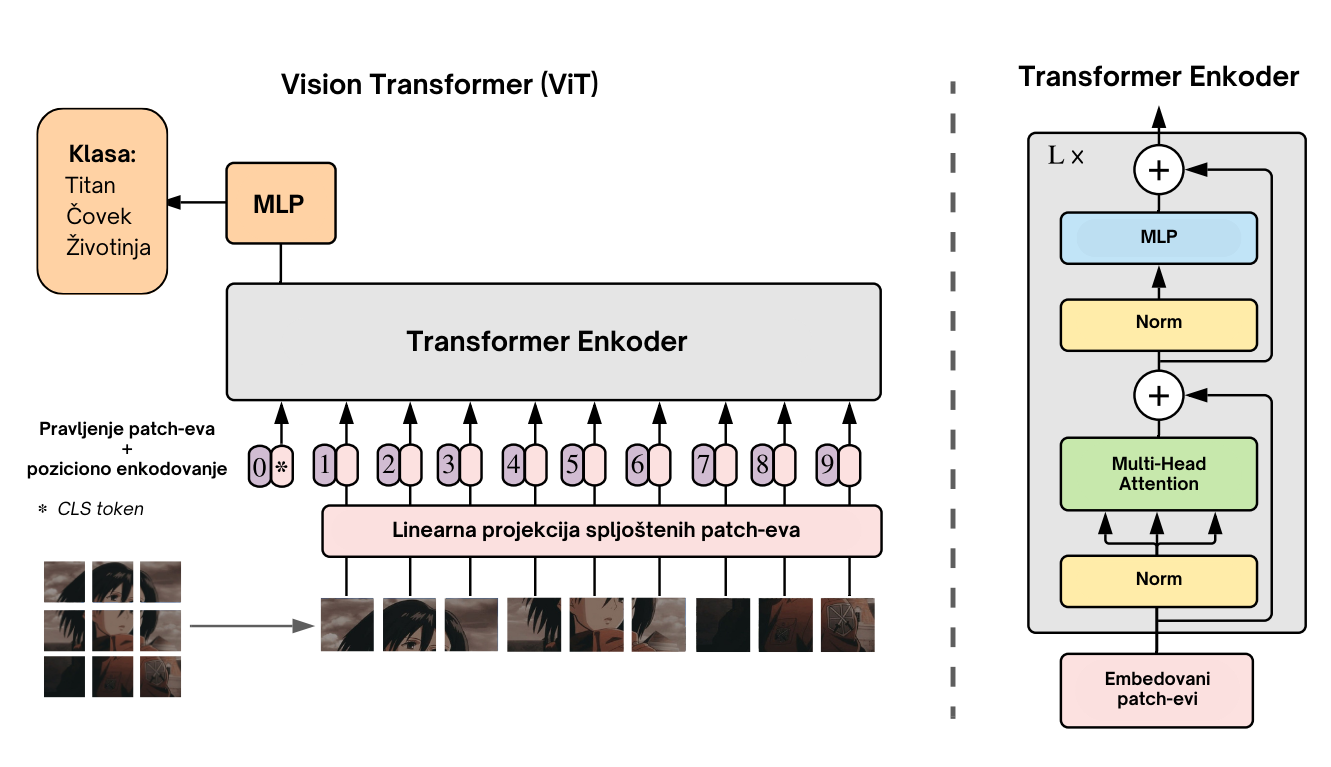
\includegraphics{vit_architecture.png}}
      \caption{Arhitektura Vision Transformera za klasifikaciju slika}
      \label{fig:vit_architecture}
   \end{figure}
   \newpage

   \subsubsection{Tokenizacija slike}
   Kod Vision Transformera, proces tokenizacije slike je ključan za prilagođavanje originalnoj arhitekturi 
   transformera, kako bi ona radila sa slikama. Za razliku od konvolucionih neuronskih mreža 
   (\textbf{CNN}), koje obrađuju slike u celini, \textbf{ViT} deli sliku na manje 
   delove poznate kao \textit{patch}-evi \cite{vit}.
   
   \subsubsection*{Deljenje slike na patch-eve}
   Prvi korak u tokenizaciji predstavlja deljenje ulazne slike na \textit{patch}-eve fiksne veličine. 
   Razmotrimo ulaznu sliku dimenzija \( H \times W \times C \), 
   gde su \( H \) i \( W \) visina i širina slike, a \( C \) je broj 
   kanala boje (obično 3 za RGB slike). Slika se deli na nepreklapajuće \textit{patch}-eve, 
   svaki veličine \( P \times P \times C \).
   
   Ukupan broj \textit{patch}-eva \( N \) dat je formulom:
   \[
   N = \frac{HW}{P^2}.
   \]
   Svaki \textit{patch} se zatim "spljošti" u jednodimenzionalni vektor 
   veličine \( P^2C \) \cite{vit_impl}.
   
   \subsubsection*{Embedobanje patch-eva}

   Nakon što je slika podeljena na \textit{patch}-eve i svaki \textit{patch} je spljošten, 
   sledeći korak je da se ovi vektori projektuju u višedimenzionalni prostor koji transformerov 
   enkoder može da obradi. Ovo se ostvaruje putem \textbf{linearne transformacije}, ovakav sloj 
   se često naziva embeding sloj (eng. \textit{patch embedding layer}).

   Za dati spljošteni \textit{patch} \( x_i \in \mathbb{R}^{P^2C} \), embeding sloj 
   ga projektuje u vektor dimenzije \( d_{model} \), gde je \( d_{model} \) dimenzionalnost 
   ulaznog prostora enkodera:

   \[
   z_i = x_i \cdot W_e + b_e.
   \]

   Ovde je \( W_e \in \mathbb{R}^{(P^2C) \times d_{model}} \) matrica težina koja se uči, 
   a \( b_e \in \mathbb{R}^{d_{model}} \) je pomeraj. Ova transformacija konvertuje svaki 
   \textit{patch} u token, vektor dimenzije \( d_{model} \), pogodan za ulaz u transformer enkoder.

   Rezultujuća sekvenca embedovanih \textit{patch}-eva formira ulaz u transformer enkoder, 
   omogućavajući modelu da obradi sliku na sličan način kao što transformer obrađuje sekvencu reči. 
   Redosled i prostorni odnosi između \textit{patch}-eva se čuvaju dodavanjem pozicionih vektora, 
   koji se sabiraju sa ovim vektorima pre nego što prođu kroz enkoder \cite{gordic}.

   \subsubsection{Poziciono Enkodovanje}
   U \textbf{ViT}-ovima, kao i u klasičnim transformerima, redosled ulaznih tokena je ključan 
   za očuvanje prostorne strukture podataka. Međutim, tokeni u \textbf{ViT} modelu sami po sebi 
   nemaju nikakvu inherentnu informaciju o poziciji, jer su rezultati deljenja slike na 
   \textit{patch}-eve. Da bi model mogao da iskoristi prostornu informaciju o \textit{patch}-evima, 
   neophodno je dodati informacije o poziciji svakom tokenu \cite{vit}.


   \subsubsection*{Fiksni pozicioni vektori}
   U \textbf{ViT} modelu, pozicioni vektori se često generišu korišćenjem sinusnih i kosinusnih 
   funkcija različitih frekvencija (isto kao i kod originalnog transformera). Za svaki 
   \textit{patch}, pozicioni vektor \( p_i \) dimenzije \( d_{model} \) se dodaje 
   vektoru \textit{patch}-a \( z_i \) kako bi se formirao finalni ulaz u Transformer enkoder:

   \[
   z_i' = z_i + p_i.
   \]

   Poziciono enkodovanje je definisano sledećim formulama:

   \[
   PE_{(pos, 2i)} = \sin\left(\frac{pos}{10000^{\frac{2i}{d_{model}}}}\right)
   \]
   \[
   PE_{(pos, 2i+1)} = \cos\left(\frac{pos}{10000^{\frac{2i}{d_{model}}}}\right)
   \]

   gde je \( pos \) pozicija \textit{patch}-a u sekvenci, a \( i \) indeks dimenzije. 
   Iako bi imalo smisla koristiti 2D poziciono enkodovanje za slike, ovaj pristup ne daje bolje
   rezultate u praksi \cite{vit}, pa se koristi jednodimenzionalni pristup.

   \subsubsection*{Pozicioni vektori koji se uče}
   Umesto korišćenja fiksnih sinusnih i kosinusnih funkcija, moguće je i da se 
   pozicioni vektori nauče tokom treniranja modela. U ovom pristupu, 
   pozicioni vektori se tretiraju kao dodatni parametri koji se optimizuju zajedno sa 
   težinama modela. Međutim, istraživanja su pokazala da fiksni pozicioni vektori daju 
   rezultate slične naučenim vektorima, dok su jednostavniji za implementaciju i računanje \cite{vit}.


   \subsubsection{Transformer Enkoder}
   \textbf{ViT} koristi arhitekturu Transformer enkodera, koja je već detaljno objašnjena. U 
   kontekstu \textbf{ViT}-a, enkoder obrađuje sekvencu tokena slike kako bi uhvatio odnose 
   i zavisnosti između različitih \textit{patch}-eva slike.

   Transformer enkoder može imati više slojeva, a sastavni deo svakog sloja su:
\begin{itemize}
   \vspace{-0.5cm}
    \item \textbf{Multi-Head Attention:} omogućava modelu da obrati pažnju na različite 
    delove slike istovremeno, modelujući složene odnose između \textit{patch}-eva,
    \item \textbf{Feedforward Neuronska Mreža:} Primenjuje se nezavisno na svaki token i 
    dalje obrađuje informacije dobijene od \textit{self-attention} mehanizma,
    \item \textbf{Rezidualne Konekcije i Normalizacija Sloja:} Ovi elementi pomažu u 
    stabilizaciji obuke i poboljšanju konvergencije normalizovanjem aktivacija i 
    uključivanjem rezidualnih konekcija.
\end{itemize}
   Izlaz iz enkodera, posebno reprezentacija \texttt{[CLS]} tokena, koristi se za zadatke klasifikacije slika \cite{vit}. 

   \newpage
   \subsubsection{Klasifikacioni MLP}
   Finalni output se dobija kroz \textit{Multi-Layer Perceptron} (MLP) glavu, koja 
   obrađuje reprezentaciju \texttt{[CLS]} token-a.

   \texttt{[CLS]} token je poseban token koji se dodaje sekvenci tokena slika pre 
   nego što se prosledi enkoderu. Njegova svrha je da agregira informacije iz svih 
   \textit{patch}-eva i služi kao kompresovana reprezentacija cele slike. Konačna 
   reprezentacija ovog tokena, nakon prolaska kroz enkoder, koristi se za 
   klasifikaciju.

   Upotreba \texttt{[CLS]} tokena u \textbf{ViT}-u je inspirisana modelom \textbf{BERT} 
   \cite{bert} u obradi prirodnog jezika, gde služi sličnu svrhu u agregaciji kontekstualnih 
   informacija za zadatke klasifikacije. Iako je \texttt{[CLS]} token pokazao svoju efikasnost u 
   \textbf{ViT}-ovima, treba napomenuti da arhitektura može funkcionisati i bez njega. 
   Alternativne metode, kao što su \textit{pooling} metode ili neke druge strategije, mogle 
   bi postići slične rezultate, ali je \texttt{[CLS]} token ostao standardan pristup zbog lakše i efikasnije
   implementacije \cite{vit}.

   \section{Eksperimenti i Rezultati}
   \subsection{Postavka eksperimenta}
   \subsubsection{Softver}
   Za potrebe eksperimenata korišćeni su:
   \begin{itemize}
      \vspace{-0.5cm}
      \setlength\itemsep{0.2em} % Set the vertical space between items
      \item \textbf{Framework:} PyTorch
      \item \textbf{Jezik:} Python
      \item \textbf{Biblioteke:} numpy, torchvision, matplotlib, seaborn
   \end{itemize}
   Upotrebljen je model sa dimenzijom tokena od 32 i 
   korišćena su 3 enkoderska bloka. \textbf{MLP} unutar enkodera imao je dimenziju 
   od 32. Brzina učenja je postavljena na 0.005, a za obuku je korišćen \textbf{Adam} 
   optimizator \cite{adam}. Veličina \textit{batch}-a bila je 128, a model je 
   treniran tokom 30 epoha. Kao funkcija gubitka korišćen je \textit{Cross entropy loss}.

   \newpage

   \subsubsection{Hardver}
   Treniranje modela je obavljeno na laptopu sa sledećom hardverskom konfiguracijom:
   \begin{itemize}
      \vspace{-0.5cm}
      \setlength\itemsep{0.2em} % Set the vertical space between items
      \item \textbf{GPU:} NVIDIA GeForce GTX 1650 Ti sa 4 GB RAM-a.
      \item \textbf{CPU:} Intel i7-10750H (12 jezgara) @ 5.000GHz.
      \item \textbf{RAM:} 64 GB.
   \end{itemize}

   Zbog resursa i vremenskih ograničenja, kao i zbog resursno intenzivne prirode 
   treniranja modela na velikim skupovima podataka, direktna poređenja sa 
   najmodernijim modelima na velikim skupovima podataka nisu bila izvodljiva. Umesto 
   toga, ovi eksperimenti se fokusiraju na implementacione detalje \textbf{ViT}-a, 
   različite delove njegove arhitekture i performanse kroz kontrolisane 
   eksperimente na manjim skupovima podataka.

   Jedan od implementacionih detalja koji je omogućio efikasno izvršavanje\footnote{Kod je dostupan na \url{https://github.com/Kovelja009/ViT_implementation}}
   jeste korišćenje PyTorch-ovih funkcija za 
   deljenje slika na \textit{patch}-eve i međusobno paralelno množenje 
   tokena unutar \textit{multi-head attention} bloka. Ove izmene su omogućile značajno 
   ubrzanje (12x do 15x) u odnosu na referentnu implementaciju \cite{vit_impl}.

   \subsubsection{Dataset}
   Eksperimenti su sprovedeni nad MNIST \cite{mnist} skupom podataka, 
   koji se sastoji od 60.000 crno-belih slika rukom pisanih cifara za obuku i 
   10.000 slika za testiranje. Svaka slika je veličine 28x28 piksela. Ovaj dataset je 
   je korišćen zbog svoje veličine i mogućnosti da se \textbf{ViT} testira na 
   zadacima manjih razmera.

   \subsection{Eksperiment 1: Poređenje fiksnih i pozicionih vektora koji se uče}
   Cilj ovog eksperimenta jeste poređenje performansi fiksnih 
   i pozicionih vektora koji se uče u pogledu preciznosti klasifikacije i 
   njihove sposobnosti da modeluju prostorne odnose na slikama.

   Rezultati:
   \begin{itemize}
      \item \textbf{Poređenje Performansi:}  Rezultati sa \textit{Slike 19} pokazuju da oba tipa vektora 
      daju sličnu preciznost klasifikacije. Međutim, pozicioni vektori koji se uče 
      pružaju nešto stabilniju preciznost kroz trening sesiju.
      \begin{figure}[h!]
         \centering
         % \hspace{-2cm} % Add horizontal space
         \vspace{1cm} % Add vertical space
         \adjustbox{scale=0.35,center}{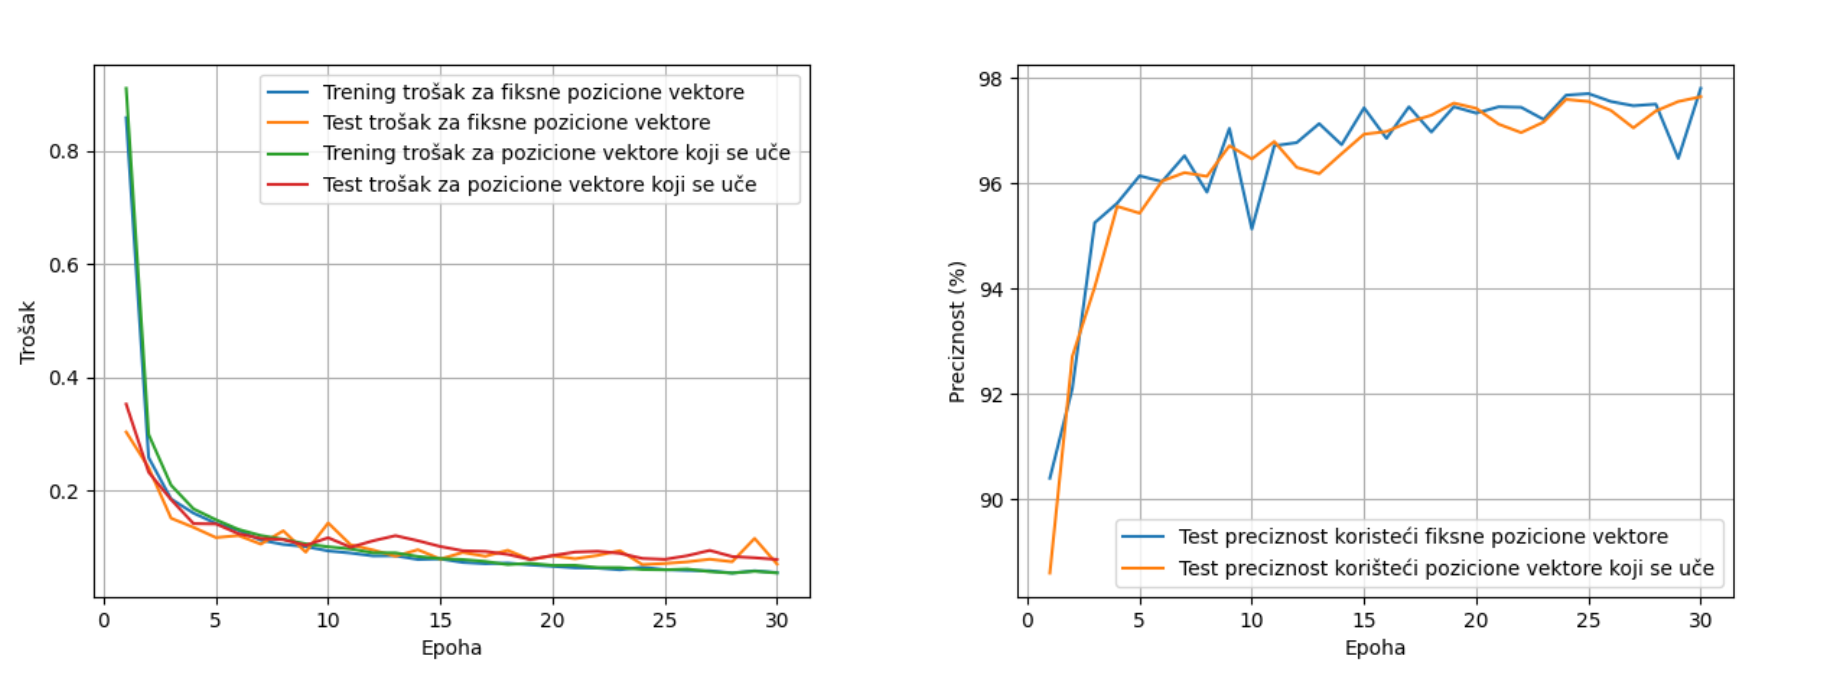
\includegraphics{exp1_metr.png}}
         \caption{Trošak tokom treninga i testa (levo) i preciznost tokom testa (desno) za fiksne i pozicione vektore koji se uče}
         \label{fig:exp1_metr}
      \end{figure}

      \newpage
      \item \textbf{Prostorni Odnosi:} \textit{Slika 20} prikazuje 
      kosinusnu sličnost između različitih delova slike. Ova analiza otkriva da 
      pozicioni vektori koji se uče modeluju prostorne odnose između delova slike tako,
      da oni na kraju podsećaju na fiksne pozicione vektore, čime je zadatak uspešno naučen.
      \begin{figure}[h!]
         \centering
         % \hspace{-2cm} % Add horizontal space
         \vspace{1cm} % Add vertical space
         \adjustbox{scale=0.25,center}{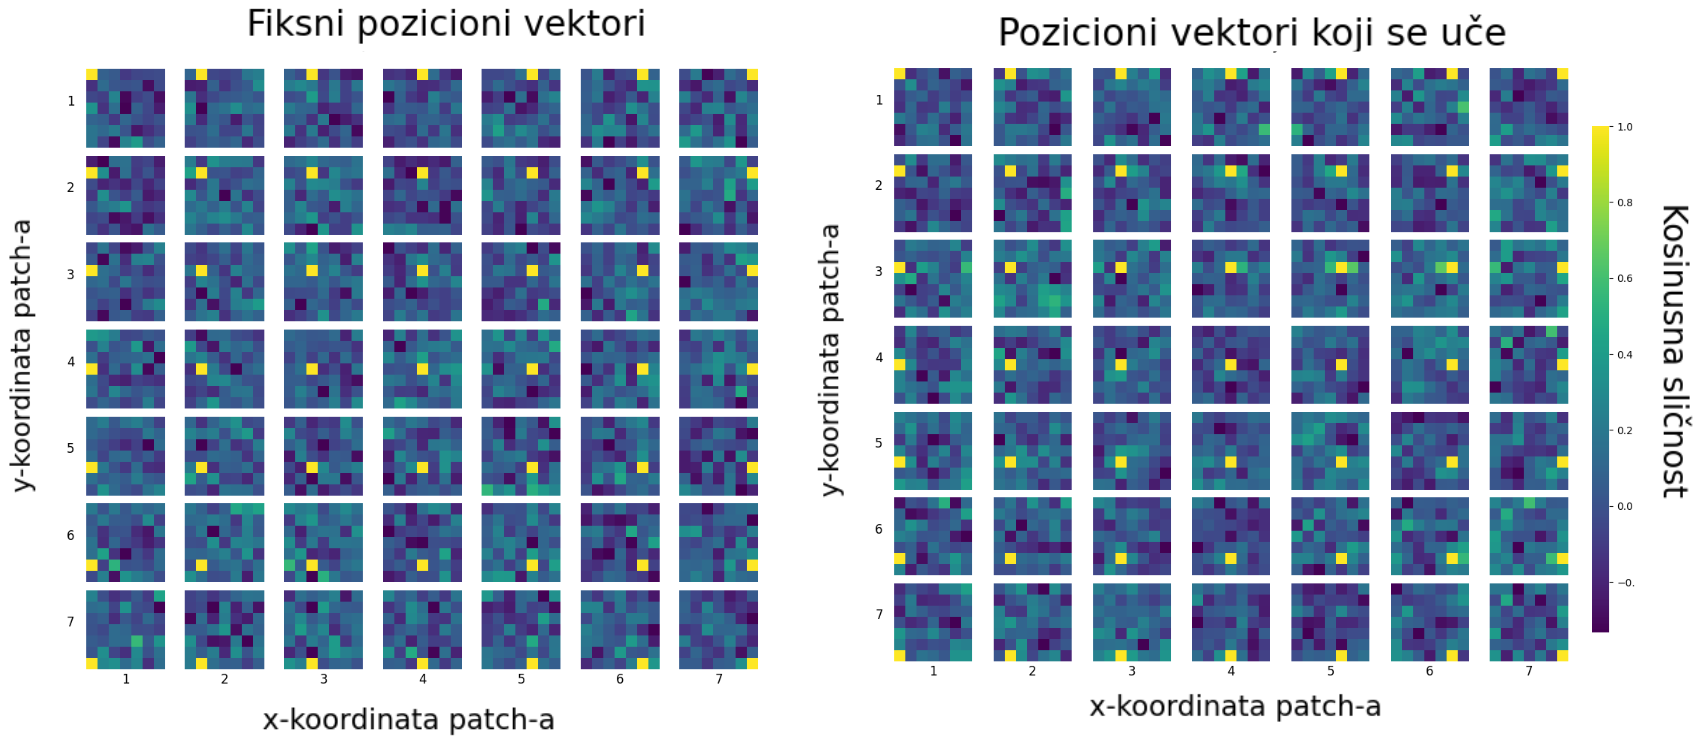
\includegraphics{exp1_cos_sim.png}}
         \caption{Kosinusna sličnost između različitih \textit{patch}-eva za fiksne i pozicione vektore koji se uče}
         \label{fig:exp1_cos_sim}
      \end{figure}
   \end{itemize}
   \newpage
   \subsection{Eksperiment 2: Uticaj uklanjanja CLS tokena}
   Cilj ovog eksperimenta je ispitivanje uticaja uklanjanja \texttt{[CLS]} tokena na 
   performanse \textbf{ViT}-a.

   \textbf{Rezultati:}
   \begin{itemize}
      \item \textbf{Performanse Modela:} \textit{Slika 21} potvrđuje da \textbf{ViT}
      ima skoro identične performanse sa i bez \texttt{CLS} tokena, što je u 
      skladu sa hipotezom koja je predstavljena u originalnom radu \cite{vit}.
      \begin{figure}[h!]
         \centering
         % \hspace{-2cm} % Add horizontal space
         \vspace{1cm} % Add vertical space
         \adjustbox{scale=0.3,center}{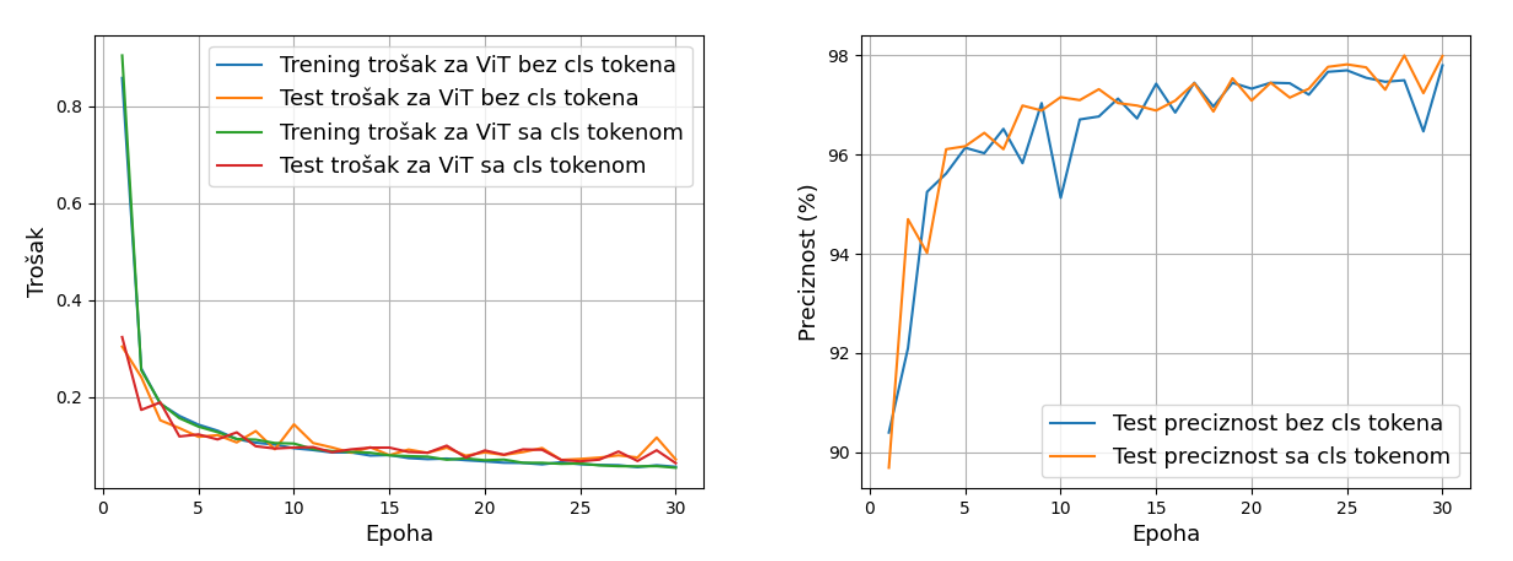
\includegraphics{exp2_metr.png}}
         \caption{Trošak tokom treninga i testa (levo) i preciznost tokom testa (desno) za modele sa i bez \texttt{CLS} tokena}
         \label{fig:exp2_metr}
      \end{figure}

      \newpage
      \item \textbf{Vreme Treninga:} \textit{Slika 22} otkriva 
      značajno smanjenje vremena treninga po epohi kada se \texttt{CLS} token izostavi 
      (približno 1.3 puta brži). Pretpostavka je da je to zbog načina 
      na koji je \texttt{CLS} token implementiran i ostaje  
      predmet dalje istrage.
      \begin{figure}[h!]
         \centering
         % \hspace{-2cm} % Add horizontal space
         \adjustbox{scale=0.7,center}{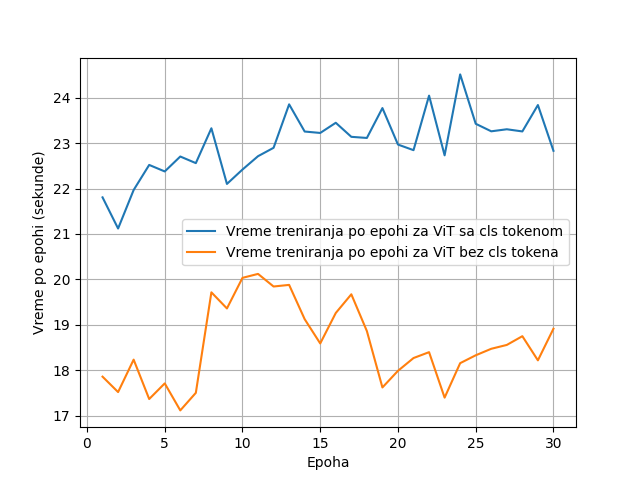
\includegraphics{training_time_cls_token.png}}
         \caption{Trošak tokom treninga i testa (levo) i preciznost tokom testa (desno) za modele sa i bez \texttt{CLS} tokena}
         \label{fig:exp2_time}
      \end{figure}
   \end{itemize}

   \newpage
   \subsection{Eksperiment 3: Uticaj veličine patch-eva na performanse}
   Cilj trećeg eksperimenta je da se proceni uticaj različitih veličina 
   \textit{patch}-eva na performanse modela. Testirane su tri veličine 
   patch-eva: 7x7, 4x4 i 2x2.

   \begin{itemize}
      \item \textbf{Performanse:} Kao što je prikazano na \textit{Slici 23}, sve tri 
      veličine \textit{patch}-eva su dale slične gubitke i preciznost tokom obuke, što ukazuje 
      na to da veličina \textit{patch}-a ne utiče značajno na sposobnost modela da uči i 
      postiže dobre performanse na \textbf{MNIST} skupu podataka. Zapažanje je da je model sa
      veličinom \textit{patch}-a 14x14 najmanje naučio u poređenju sa početnim epohama. Intuicija
      je da se model preprilagođava pošto je \textit{patch} veliki (2x2 ukupan broj \textit{patch}-eva), pa
      je bolje koristiti manje \textit{patch}-eve. 
      \begin{figure}[h!]
         \centering
         % \hspace{-2cm} % Add horizontal space
         \vspace{1cm} % Add vertical space
         \adjustbox{scale=0.3,center}{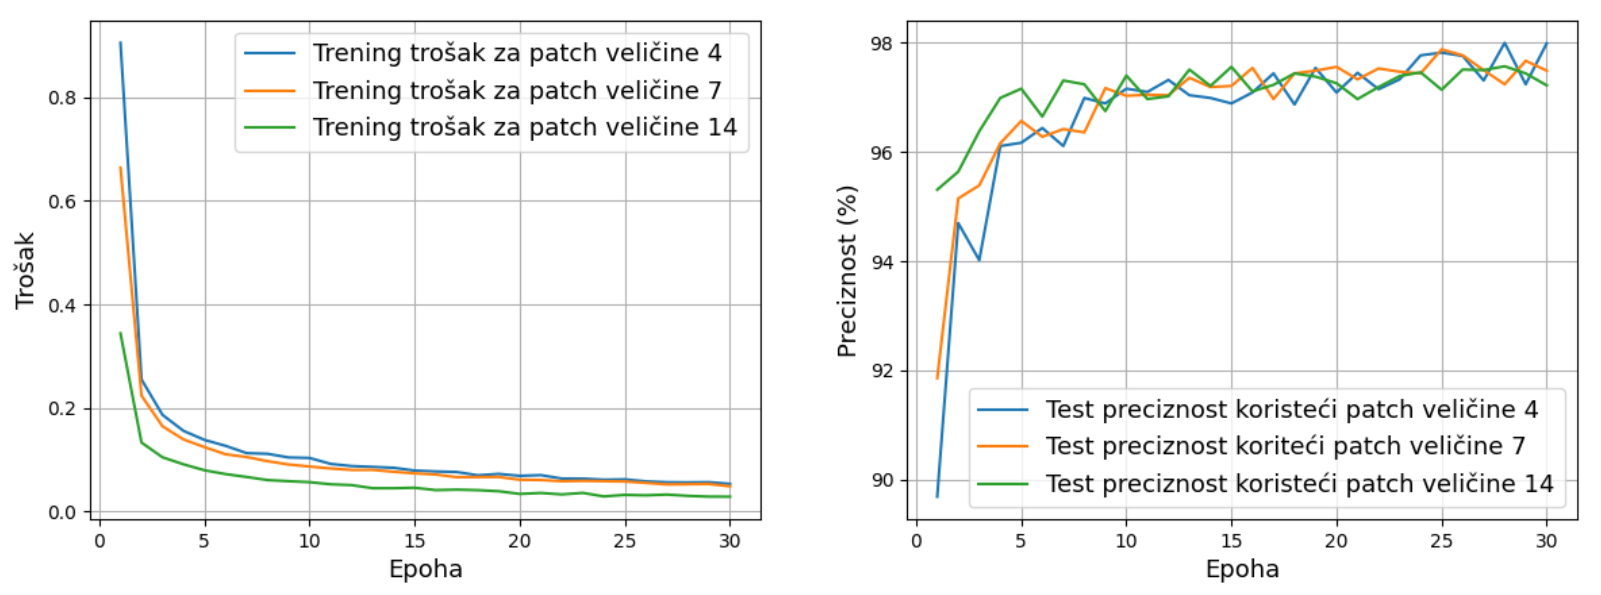
\includegraphics{exp3_metr.png}}
         \caption{Trošak tokom treninga (levo) i preciznost tokom testa (desno) za modele sa različitom veličinom patch-eva}
         \label{fig:exp3_metr}
      \end{figure}

      \newpage
      \item \textbf{Vreme obuke:} \textit{Slika 24} otkriva zanimljivo zapažanje: 
      \textit{patch}-evi veličine 14 (2x2) imali su najsporije vreme obuke po epohi. 
      Razlog za to može biti posledica implementacije linearnog \textit{embedding} sloja, 
      mada su potrebna dodatna ispitivanja da bi se ova hipoteza potvrdila.
      \begin{figure}[h!]
         \centering
         % \hspace{-2cm} % Add horizontal space
         % \vspace{-0.5cm} % Add vertical space
         \adjustbox{scale=0.7,center}{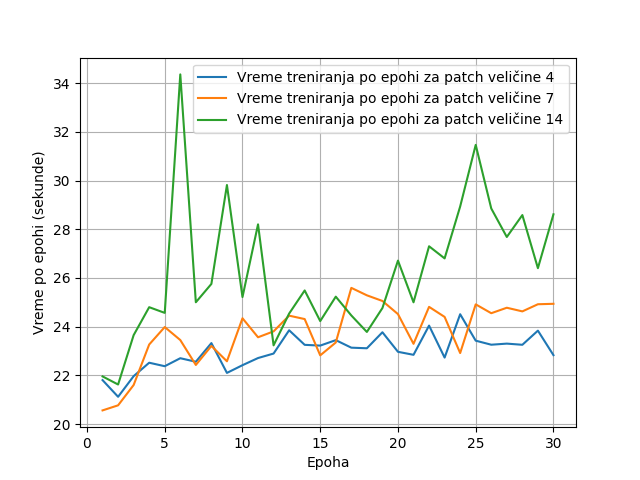
\includegraphics{patches_times.png}}
         \caption{Vreme obuke po epohi za različite veličine \textit{patch}-eva}
         \label{fig:exp3_time}
      \end{figure}
   \end{itemize}
   \newpage
   \section{Zaključak}

   U radu je detaljno objašnjena arhitektura Vision Transformer modela, uključujući 
   proces pretvaranja slika u tokene, korišćenje enkodera, i značaj klasičnog 
   transformer modela.

   Kroz implementaciju i eksperimentalne rezultate, pokazano je da \textbf{ViT} modeli 
   mogu uspešno da obrade slike i postignu konkurentne rezultate.

   Eksperimenti su obuhvatili upotrebu fiksnih nasuprot pozicionim vektorima koji se uče, 
   uticaj uklanjanja \texttt{[CLS]} tokena na performanse modela, i analizu uticaja 
   veličine \textit{patch}-eva na vreme obuke i preciznost modela.

   Rezultati su pokazali da fiksni i pozicioni vektori koji se uče imaju slične 
   performanse, dok je uklanjanje \texttt{[CLS]} tokena imalo minimalan uticaj na 
   performanse, ali je značajno smanjilo vreme obuke. Takođe, veličina \textit{patch}-eva 
   ima uticaj na vreme obuke, s manjim \textit{patch}-evima koji mogu da 
   unaprede efikasnost modela.

   Potencijalni fokus budućih istraživanja bi bio na isprobavanju alternativnih strategija 
   za modelovanje globalnog konteksta bez oslanjanja na \texttt{[CLS]} token. Ovo može 
   uključivati eksperimentisanje sa različitim \textit{pooling} strategijama. Takođe, 
   vizualizacija \textit{attention} mapa tokom procesa klasifikacije mogla bi pružiti uvide u 
   delove slike na koje se enkoder fokusira, što bi dovelo do bolje interpretabilnosti modela.

   \newpage
   \printbibliography[title={Literatura}]
\end{document}